\documentclass[12pt,a4paper]{report}
%\linespread{1.3}
\usepackage{fullpage}
\usepackage{setspace}

\usepackage{pifont,multirow}
\usepackage{enumitem}
\usepackage{graphics,graphicx,url, wrapfig,latexsym,epsfig}
\usepackage{hyperref,fancyhdr,comment,epic}
\usepackage{amsmath,algorithm}
\usepackage{algpseudocode}
\usepackage{makeidx,setspace}
\usepackage{longtable}
\usepackage{mdwmath,mdwtab}
\usepackage{stfloats}
\usepackage{fontspec,verbatim}
\usepackage[titletoc]{appendix}
\usepackage[stable]{footmisc}
\usepackage{listings}
\usepackage{xcolor}
%---------------------------------------------------------------------
\interfootnotelinepenalty=10000
%---------------------------------------------------------------------
\font\en="Latin Modern Roman Unslanted:script=roman" at 12pt
\font\ens="Latin Modern Roman Unslanted:script=roman" at 12pt
\font\ipa="Doulos SIL:script=roman" at 11pt
\font\ipas="Doulos SIL:script=roman" at 9pt

%----------------------------------------------------------------------
\graphicspath{{figures/}}
\setlength{\parskip}{1mm}
\setlength{\lineskip}{1mm}
\setlength{\parindent}{20pt}
\hypersetup{
    bookmarks=true,         % show bookmarks bar?
    unicode=true,          % non-Latin characters in Acrobat’s bookmarks
    pdftoolbar=true,        % show Acrobat’s toolbar?
    pdfmenubar=true,        % show Acrobat’s menu?
    pdfauthor={RadheTians},     % author
    colorlinks=true,       % false: boxed links; true: colored links
    linkcolor= blue,          % color of internal links
    citecolor=magenta,        % color of links to bibliography
    filecolor=cyan,      % color of file links
    urlcolor=magenta           % color of external links
}
%-------------------------------------------------------------------
\newcommand{\FF}{\vspace*{\medskipamount}}
\newcommand{\act}[1]{\mbox{#1}}
\newcommand{\sglspc}{\renewcommand{\baselinestretch}{1.00}\normalsize}
\newcommand*\circled[1]{\tikz[baseline=(char.base)]{%
            \node[shape=circle,draw,inner sep=1pt] (char) {#1};}}

\makeatletter
\newenvironment{tablehere}{\def\@captype{table}}{}
\newenvironment{figurehere} {\def\@captype{figure}}{}
\makeatother

\newcommand{\newphases}{\setcounter{phase}{0}}
\newcommand{\phase}[1]{\vspace{1 ex}\addtocounter{phase}{1}\par\noindent{\bf \Alph{phase} #1}}
\newcommand{\phaselabel}[1]{\newsavebox{#1}\sbox{#1}[\Alph{phase}]}
\newcommand{\phaseref}[1]{\usebox{#1}}
%------------------------------------------------------------------------
\makeindex
\newcolumntype{L}{>{\arraybackslash}m{5.7cm}}
\newcolumntype{T}{>{\arraybackslash}m{2.3cm}}
%------------------------------------------------------------------------
\setlength{\arrayrulewidth}{1mm}
\setlength{\tabcolsep}{18pt}
\renewcommand{\arraystretch}{1.5}
%------------------------------------------------------------------------
\definecolor{codegreen}{rgb}{0,0.6,0}
\definecolor{codegray}{rgb}{0.5,0.5,0.5}
\definecolor{codepurple}{rgb}{0.58,0,0.82}
\definecolor{backcolour}{rgb}{0.95,0.95,0.92}

\lstdefinestyle{codeStyle}{
    backgroundcolor=\color{backcolour},   
    commentstyle=\color{codegreen},
    keywordstyle=\color{magenta},
    numberstyle=\tiny\color{codegray},
    stringstyle=\color{codepurple},
    basicstyle=\ttfamily\footnotesize,
    breakatwhitespace=false,         
    breaklines=true,                 
    captionpos=b,                    
    keepspaces=true,                 
    numbers=left,                    
    numbersep=5pt,                  
    showspaces=false,                
    showstringspaces=false,
    showtabs=false,                  
    tabsize=2
}
\lstset{style=CodeStyle}
%---------------------------------------------------------------------
\begin{document}
\pagenumbering{roman}
\thispagestyle{empty}
\begin{center}

\vspace*{1.2 cm}
{\Huge{\bf AIR POLLUTION DETECTOR}}

\vspace{0.3 in}
{\en A final report submitted for the course named Project II(CS-300)}


\vspace{0.5 in}
{\it BY\\}	
\vspace{0.2 in}
{\Large \bf RADHE RAMAN TIWARI\\}
\vspace{0.2 in}
{\bf Bachelor of Technology, VI Semester\\}
\vspace{0.2 in}
{\bf Roll No. 17010115}\\
\vspace{0.5 in}
{\it Under the Supervision and Guidance of\\}
\vspace{0.2 in}
{\Large \bf Dr. NAVANATH SAHARIA}\\

\vspace{0.9 in}

\includegraphics[scale=0.95]{iiitm-logo.png}
\vspace{0.8 in}

{\large\bf Department of Computer Science and Engineering\\}
\vspace{0.2 in}
{\Large\bf Indian Institute of Information Technology Manipur\\}
\vspace{0.1 in}
{\large June, 2020 }

\end{center}


\chapter*{Abstract}
\addcontentsline{toc}{chapter}{\numberline{}Abstract}
\bigskip
\begin{onehalfspace}
{\en Air pollution affects our day to day activities and quality of life. It poses a threat to the ecosystem and the quality of life on the planet. The dire need to monitor air quality is very glaring, owing to increased industrial activities over the past years. People need to know the extent to which their activities affect air quality. This project proposes an air pollution monitoring system. The system is developed using the Raspberry Pi 4 and Arduino UNO micro-controller. The air pollution monitoring system is designed to monitor and analyze air quality in real-time and log data to a remote server, keeping the data updated over the internet. Air quality measurements are taken based on the Parts per Million (PPM) metrics and analyzed using Flutter application. The air quality measurements taken by the designed system is accurate.The result is displayed on the designed Flutter application (which runs both on Android and iOS) and the prediction of next few days weather forecast based on past data using supervised Machine Learning approach.


} 
\end{onehalfspace}




\bigskip

\noindent{\bf Keywords} - {\en Raspberry Pi 4, Arduino UNO, IOT, Pollution,  AQI, PPM, Flutter, Firebase, Python3, Gas Sensors.}




\chapter*{Declaration}
\addcontentsline{toc}{chapter}{\numberline{}Declaration}



%\centerline{\Large\bf Declaration }

\vspace*{6 ex}
{\ens
I declare that this submission represents my idea in my own words and where others' idea or words have been included, I have adequately cited and referenced the original source. I also declare that I have adhered to all principles of academic honesty and integrity and have not misrepresented or fabricated or falsified any idea/data/fact/sources in my submission. I understand that any violation of the above will be a cause for disciplinary action by the institute and can also evoke penal action from the sources which have thus not been properly cited or from proper permission has not been taken when needed.

\vspace*{10 ex}

\begin{tabular}{p{10.0 cm}p{7.0 cm}@{}}
%& \\ \cline{2-2}

&\multicolumn{1}{r@{}}{(Signature)}\\ 
& \\ \cline{2-2}

&\multicolumn{1}{r@{}}{(Name of the student)}\\
& \\ \cline{2-2}
Date: &\multicolumn{1}{r@{}}{(Roll no)}\\
%& \\ \cline{2-2}
\end{tabular}
}


%\addcontentsline{toc}{chapter}{\numberline{}Certificate}
%\thispagestyle{empty}
\singlespacing
\parindent 0pt
\parskip 3pt


\begin{tabular}{cl}
\multirow{2}{*}{
\includegraphics[scale=0.60]{iiitm-logo.png}} &{\large Department of Computer Science \& Engineering}\\
&{\large Indian Institute of Information Technology Manipur}\\
%&{\large \bf Transit Campus, Mantripukhri, Imphal, India - 795002}\\ 
&\noindent\rule{12cm}{1.5pt}\\
&Dr. XYZ ABC \hfill 	Email: xyzx@iiitmanipur.ac.in\\
&Assistant Professor \\
\end{tabular}

\vspace{3.5cm}
\hbox{\centerline{\Large{\bf To Whom It May Concern}}}
\vspace{1.8cm}
\parindent 40pt
\parskip 12pt


{\en
\noindent
This is to certify that the report entitled {\bf ``TITLE of THE report"} submitted to by "Name of the student", has been carried out under my supervision and that this work has not been submitted elsewhere for a degree,diploma or a course.

\vspace{0.8 in}


\begin{flushright}
Signature of Supervisor\\ 
\vspace{0.8in} 
(Dr. XYZ)\\
\end{flushright}
}





%\addcontentsline{toc}{chapter}{\numberline{}Certificate}
%\thispagestyle{empty}
\singlespacing
\parindent 0pt
\parskip 3pt


\begin{tabular}{cl}
\multirow{2}{*}{
\includegraphics[scale=0.60]{iiitm-logo.png}} &{\large Department of Computer Science \& Engineering}\\
&{\large Indian Institute of Information Technology Manipur}\\
%&{\large \bf Transit Campus, Mantripukhri, Imphal, India - 795002}\\ 
&\noindent\rule{12cm}{1.5pt}\\
\end{tabular}

\vspace{3.5cm}
\hbox{\centerline{\Large{\bf To Whom It May Concern}}}
\vspace{1.8cm}
\parindent 40pt
\parskip 12pt


{\en
\noindent


\vspace{0.8 in}

\begin{flushright}
Signature of HoD\\ 
\vspace{0.8in} 
(Dr. XYZ)\\
\end{flushright}
}
\vspace{0.3 in}
\begin{flushleft}
Signature of Examiner 1: \rule{5cm}{1.5pt}\\ 
\vspace{0.7in}
Signature of Examiner 2: \rule{5cm}{1.5pt}\\ 
\vspace{0.7in}
Signature of Examiner 3: \rule{5cm}{1.5pt}\\
\end{flushright}
}








\chapter*{Acknowledgement}
\addcontentsline{toc}{chapter}{\numberline{}Acknowledgement}

\thispagestyle{empty}


{\en


I extend my sincere thanks to the institute \textbf{Indian Institute of Information Technology Senapti, Manipur} who has provided me an opportunity to do the project. I would like to express deep dept to Dr. Navnath Saharia , project guide for his vital suggestion ,meticulous guidance and constant motivation which went a long way in successful completion of the project. I cannot move forward without thank to  Dr. Nongmeikapam Kishorjit Singh and Dr. Prerna Mohit who has always been an inspiration to me. I would
like to thanks to Dr.Kabita Tharoijam, project co-ordinator who has been organizing the
project presentation time to time which helped me to finish the project on time. On a moral personal note my deepest appreciation and gratitude to my beloved friends ,who has been an inspiration and have provided me a unrelenting encouragement and support

}
\begin{flushright}

{\en - Radhe Raman Tiwari\\ 17010115}
\end{flushright}


\cleardoublepage\phantomsection
\setcounter{secnumdepth}{4}
\setcounter{tocdepth}{4}

\addcontentsline{toc}{chapter}{\numberline{}Table of contents}
\tableofcontents



\cleardoublepage\phantomsection\addcontentsline{toc}{chapter}{\numberline{}List of tables}
\listoftables


\cleardoublepage\phantomsection\addcontentsline{toc}{chapter}{\numberline{}List of figures}
\listoffigures

\lstlistoflistings

%\chapter*{List of abbreviations}
\addcontentsline{toc}{chapter}{\numberline{}List of abbreviations}

{\centering
\begin{longtable}{@{}p{2 cm}@{}p{2 cm}@{}p{11 cm}@{}}
\multicolumn{3}{r}{\bf A}\\ \cline{2-3}
&ASCII&American Standard Code for Information Interchange\\
&&\\


\multicolumn{3}{r}{\bf C}\\ \cline{2-3}
&CFG&Context Free Grammar\\
&CRF&Conditional Random Fields\\
&&\\

\multicolumn{3}{r}{\bf D}\\ \cline{2-3}
&DB&Database\\
&DBMS&Database Management Systems\\
&&\\




\multicolumn{3}{r}{\bf H}\\ \cline{2-3}
&HTML &Hyper Text Mark-up Language \\
&HMM&Hidden Markov Model \\
&&\\

\multicolumn{3}{r}{\bf I}\\ \cline{2-3}
&IPA&International Phonetics Alphabets\\
&IR& Information Retrieval\\
&&\\

\multicolumn{3}{r}{\bf M}\\ \cline{2-3}
&MLP&Multilayer Perceptron\\
&MST &Maximum Spanning Tree parser \\
&&\\

\multicolumn{3}{r}{\bf X}\\ \cline{2-3}
&XML&Xtended Mark-up Language\\


\end{longtable}}


\pagenumbering{arabic}
\setcounter{page}{1}
%\newpage\null\thispagestyle{empty}\newpage
\begin{onehalfspace}
\chapter{Introduction}\label{chap1}


%##########################################

\vspace{2in}
\begin{center}
	\textbf{\large "Be A Part OF The Solution Not Part OF The Pollution"}
\end{center}


\newpage

Air is one of the essential elements of man’s surroundings. The earth’s atmosphere is full of air which contains gases such as Nitrogen, Oxygen, Carbon Monoxide and traces of some rare elements. Humans need an atmosphere of air that is free from contaminants. This is very crucial for human life and health. Any change in the natural composition of air may cause grave harm to life forms on earth. Air pollution is the presence of one or more contaminants in the atmosphere such as gases in a quantity that can harm humans, animals and plant . Air pollutants are measured in Parts per Million (ppm) or ug/m3. Primary pollutants are released directly into the atmosphere. Secondary pollutants are produced when the primary pollutant reacts with other atmospheric chemicals . Air quality affects public health. The effect of air pollution ranges from difficulty in breathing, coughing, aggravation of asthma and emphysema. Polluted air can also impair visibility. Air pollution is accountable for the death of 7 million persons worldwide each year or one in eight premature deaths yearly . Almost 570,000 children under the age of five die every year from respiratory infection linked to indoor/outdoor pollution and second-hand smoke. Children exposed to air pollution have an elevated risk of developing chronic respiratory problems such as asthma. In the monitoring of air pollution, several researchers worldwide have developed models to monitor many of the pollution gases such as Sulphur Dioxide (SO2), Carbon Monoxide (CO), Carbon Dioxide (CO2), Nitrogen Oxides (NO) etc. This thesis project focuses on the design and implementation of a smart air pollutant monitoring system. It discusses how the level of pollutants in the air can be monitored using a gas sensors, Raspberry Pi 4 \& Arduino UNO micro-controller. The main objective of this project is to design a smart air pollution monitoring system that can monitor, analyse and log data about air quality to a remote server, keep the data up to date over the internet and predict weather forecast of next few days based on past data.



%########################################################
\section{Outline of the report}
This report is organised around three main parts. 

{\bf Chapter~\ref{chap1}} Introduction to the project 

{\bf Chapter~\ref{chap2}} Describes literature review
    
{\bf Chapter~\ref{chap3}} Describes system design \& methodology of the project

{\bf Chapter~\ref{chap4}} Describes implementation \& testing of project

{\bf Chapter~\ref{chap5}} Conclusion

\section{Problem Statement}
The aim of this thesis project is to fulfill the following goals.

\begin{enumerate}
\item Create a system which will monitor the quality of air of our environment.
\item Collect information about the air pollution level after every certain period.
\item Content of different gases present in air or area around us.
\item To collect information about the air pollution level after every certain period.
\item Sense how much amount of gasses are present in air and display it in real time on smartphone.
\item Send the information of current air pollution level and weather forecast of next upcoming days to user smartphone.
\end{enumerate}

\section{Gantt Chart}

For proper completion of any work, there is need of a proper plan and the division of the work into small time frames. I divided my work according to the following Gantt Chart.

\begin{table}[!ht]
\centering
\begin{tabular}{ |p{4cm}|p{4cm}|p{4cm}|  }
\hline
\multicolumn{3}{|c|}{Air Pollution Detector} \\
\hline
20 Jan - 20 Feb  &  21 Feb - 12 April  &  05 April - 20 April  \\
\hline
& & \\
Planning, Setup and Literature Review& & \\
& & \\
&Designing and Implementation & \\
& & \\
& & Testing and Report-Writing  \\
& & \\
\hline
\end{tabular}
\caption{\label{ganthchart}Gantt chart}
\end{table}

\section{Internet of Things(IOT)}

Internet of Things (IOT) is a network of devices that connect directly with each other to capture and share data through a secure service layer that connects to a central command and control server in the cloud. The closure look suggest that the way people collect, record and analyze data not just in health care but in every industry today. The idea of devices connecting directly with each other is basically called Internet of Things.

The Internet of Things also called the Internet of Objects, refers to a wireless network between objects, usually the network will be wireless and self-configuring. Internet of Things (IOT) is one of the major component advances in present time that links the internet with everyday sensor and working devices. Smart objects play an important role in the Internet of Things vision, since embedded communication and information technology would have the potential to change the utility of these objects. Using sensors they are able to recognize their condition, and via built-in connecting power they would be able to interact with each other.

Internet of Things (IOT) came into existence in 2009. It encircles the idea of connecting all gadgets and devices to the internet. The concept of Internet of Things is actually trying to change our world by connecting everything with each other. It is basically making our health, and businesses, society by developing products which would lead to a comfortable life. By 2020 it is estimated that, about 50 billion devices would be linked to the Internet and the market would be worth around 14 trillion USD.

IOT in different application domains alike web property of everyday objects may be accustomed remotely confirm their state in order that we will perpetually collect the info and knowledge on physical objects and processes. This qualifies several options of the
important world to be spot at a antecedently unattained level of detail and at terribly low value nearly too negligible. This could not afford an improved understanding of the underlying processes, however additionally for a lot of economical management and management. The potential to react to events during this world in associate automatic manner not solely disclose new opportunities for addressing composite or unfavorable
things, however additionally allows a large type of business processes to be optimized.

\section{Air Pollution}

Air pollution occurs when harmful or excessive quantities of substances are introduced into Earth's atmosphere. Sources of air pollution include gases (such as ammonia, carbon monoxide, sulfur dioxide, nitrous oxides, methane and chlorofluorocarbons), particulates (both organic and inorganic), and biological molecules. It may cause diseases, allergies and even death to humans; it may also cause harm to other living organisms such as animals and food crops, and may damage the natural or built environment. Both human activity and natural processes can generate air pollution.

Air pollution is a significant risk factor for a number of pollution-related diseases, including respiratory infections, heart disease, COPD, stroke and lung cancer. The human health effects of poor air quality are far reaching, but principally affect the body's respiratory system and the cardiovascular system. Individual reactions to air pollutants depend on the type of pollutant a person is exposed to, the degree of exposure, and the individual's health status and genetics. Indoor air pollution and poor urban air quality are listed as two of the world's worst toxic pollution problems in the 2008 Blacksmith Institute World's Worst Polluted Places report. Outdoor air pollution alone causes 2.1 to 4.21 million deaths annually. Overall, air pollution causes the deaths of around 7 million people worldwide each year, and is the world's largest single environmental health risk.



 %Introduction
\chapter{Literature Review}
\label{chap2}
%##########################################


\vspace*{45 ex}
%##########################################



\paragraph*{Outline:} This chapter presents the following:
\begin{enumerate}
\setlength{\itemsep}{-0.3em}
\item Efficient Noise and Air Pollution Monitoring System
\item IOT Based Air Pollution Monitoring System 
\item IOT Based Air and Noise Pollution Monitoring using Raspberry Pi
\item Air Pollution Monitoring System Using Mobile GPRS Sensors
\item Embedded device for measuring noise and air levels in atmosphere
\item IOT Based Air and Noise Pollution Monitoring in Urban and Rural Areas
\end{enumerate}


%+++++++++++++++++++++++++++++++++++++++++++++++++++++++++++++++++
\newpage
% \section{Introduction}
% Research in science and technology has played a vital role in improvising human life at great extent. With the development of instrumentation and computation facilities, research on frontier areas~\cite{bohmova+03} has gone manifold. The discussion on the frontier areas of research~\cite{collins03} in inter- disciplinary subject has always yielded novel ideas and collaborative research. In view of this, the First International Conference on Smart Technologies in Computer and Communication~\cite{choudhury07} (SmartTech-2017) is meticulously planned to muster innovative ideas from researchers, scientists, academicians, Industry professionals and students. The aim of the conference is to provide a common platform to share and discuss the novel ideas, technologies and research findings to promote interdisciplinary research and to ignite young brains.

% \begin{figure}[!ht]
% \centering
% \includegraphics[scale=0.9]{car2.png}
% \caption{\label{img2} Image caption}
% \end{figure}

% Description of Figure~\ref{img2}. .... 
% Research in science and technology has played a vital role in improvising human life at great extent. With the development of instrumentation and computation facilities, research on frontier areas has gone manifold. The discussion on the frontier areas of research in inter- disciplinary subject has always yielded novel ideas and collaborative research. In view of this, the First International Conference on Smart Technologies in Computer and Communication (SmartTech-2017) is meticulously planned to muster innovative ideas from researchers, scientists, academicians, Industry professionals and students. The aim of the conference is to provide a common platform to share and discuss the novel ideas, technologies and research findings to promote interdisciplinary research and to ignite young brains~\cite{bharati+09}.

% \section{SomayyaMadakam, R. Ramaswamy “Internet of Things”(2015)}
% This paper deals with that future is Internet Of Things, which will modify the real world things into intelligent practical things. Internet of Things works on the principal to unite everything in our world under same infrastructure, giving us not only control of object around us, but also keeping us informed of the condition of the object. The objective of this paper is to deliver an abstract of Internet of Things, architectures and essential technologies and their researchers, who wants to do research in the field of Internet of Things. 


\section{AnjaiahGuthi “Efficient Noise and Air Pollution Monitoring System” (2016)}
This paper deals with smart sensor network that are an emerging field of research which combines many challenges of computer science, wireless communication and electronics. In this research paper a solution for monitoring the noise and air pollution levels in industrial environment or any other area of interest using wireless embedded computing system is proposed.

The running representation of the initiated hardware is evaluated using original implementation, consisting of Arduino hardware support package. The hardware is tested for two or three parameters like noise, CO2 and radiation levels with respect to the normal behavior levels or given specification which provide a control over the pollution monitoring to make the environment smart.



\section{PalaghatYaswanthSai(2017)}
This document deals with the IOT Based Air Pollution Monitoring System in which we will gather the air value in PPM(Parts Per Million) as well as sound value in decibel over a web using internet and with the help of Wi-Fi module and will trigger an alarm when the air quality goes down further a certain level, means when there are sufficient amount of harmful gases are present in the atmosphere like CO2, smoke, alcohol, benzene and NH3. It will show the air quality in PPM on the LCD 16x2 display and as well as on web so that we can gather information very easily. In this MQ-135 gas sensor is used which is the best choice for monitoring air quality as it can detect most harmful gases and can measure their value efficiently. In this project, you can gather the level of air pollution and noise from anywhere using your computer or mobile. System can be set anywhere in the world and we can also activate some objects like for example when pollution goes beyoud some set level we can switch on the exhaust fan.

\section{Uppugunduru Anil Kumar, G Keerthi (2017) IOT Based Air and Noise Pollution Monitoring using Raspberry Pi}

A systematic environment monitoring hardware is required to monitor the conditions in case of exceeding the level of parameters(e.g., noise, CO2). When the things like environment equipped with sensor devices, micro-controller and various software applications becomes a self-protecting and self-monitoring environment. People need different types of monitoring hardware which are depends on the type of data monitored by the sensor. Event Detection based and Spatial Process Estimation are the two categories to which applications are classified. Initially the sensor devices are deployed in environment  to detect the parameters(e.g., noise, CO, and radiation levels etc.) which the data acquisition, computation and controlling action e.g., the variations in the noise and CO level with respect to the specified levels). Sensor devices are placed at different location to collect the data to predict the behaviour of a particular area of interest. The main focus of the this document is to model and implement an efficient monitoring
hardware through which the required values are measured remotely using web and the
information gathered from the sensors are stored in the cloud and to project the estimated
trend on the web browser.

\section{Ashvini S .kale in Air Pollution Monitoring System Using Mobile GPRS Sensors}
This paper contains brief introduction to vehicular pollution. The proposed system consists of a transmitter and receiver part. The transmitter part is integrated with single chip micro-controller, air pollution sensors array a General Packet Radio Service Modem (GPRS Modem) and a Global Positioning System Module (GPS Module) for transmitting the information.

\section{L.Ezhilarasi, K.Sripriya, “A SYSTEM FOR MONITORING AIR AND SOUND
POLLUTION USING ARDUINO CONTROLLER WITH IOT TECHNOLOGY”
(2017)}

The document contains embedded device for measuring noise and air levels in atmosphere and to make the environment in intelligent or interactive with things. The proposed model is flexible and distributive in nature to measure the environmental parameters. The architecture is developed for noise and air pollution monitoring Smart sensor network are the coming field of research and investigation which may lead to many challenges of computer science, wireless communication and electronics.

\section{Dr. Siva yellampalli “IOT Based Air and Noise Pollution Monitoring in Urban
and Rural Areas, Important Zones like Schools and Hospitals in Real Time” (2017)}

Today's major environment \& public issue is air pollution. According to the report of World Health Organization(WHO), air pollution is significant risk factor for multiple health conditions including skin \& eye infection, irritation of nose, throat \& eyes. It also causes serious condition like heart disease, lung cancer difficulty in breathing \& many. Parking management is also main public issue in most of metropolitan cities and that is also the reason of many problems. The main objective of project is by using various sensors, GSM/GPRS module and Cloud/server to design an efficient and remote system to monitoring the level of various pollutants causing pollution and to minimize the effect of these parameters without affecting the natural environment and provide live updates to avoid conflicts.  
 %Background study
\chapter{System Design, Methodology}\label{chap3}

%##########################################
\vspace*{50 ex}

%##########################################
\paragraph*{Outline:} This chapter presents the following:
\begin{enumerate}
\setlength{\itemsep}{-0.3em}
\item A brief of system design
\item A brief of methodology
\end{enumerate}
\newpage



\section{System Design }


The simplified diagram of the proposed system is
demonstrated in Fig.\ref{img31}. Raspberry pi is the major node
controlling our system. The sensors are being used for
detecting different environmental parameters like particulate
matter, Carbon Monoxide, Carbon Dioxide, Temperature,
Humidity and Pressure. The sensors are connected to Arduino
Board and Raspberry pi is interfaced with Arduino Uno
through USB cable. The data sensed by the sensors are
continuously transmitted through Raspberry pi to the cloud
over the internet because of its good network connectivity.
The sensors DSM501A is a PM sensor whose output is PWM,
used for measuring the particulate matter i.e. smoke and dust
present in our environment, DHT11 and BMP180 are having
digital outputs used for measuring temperature, humidity and
pressure. The sensors, MQ9 (Gas sensor) as well as
MQ135(air quality sensor) are analog sensors used for
measuring Carbon monoxide and carbon dioxide.

\begin{figure}[!ht]
\centering
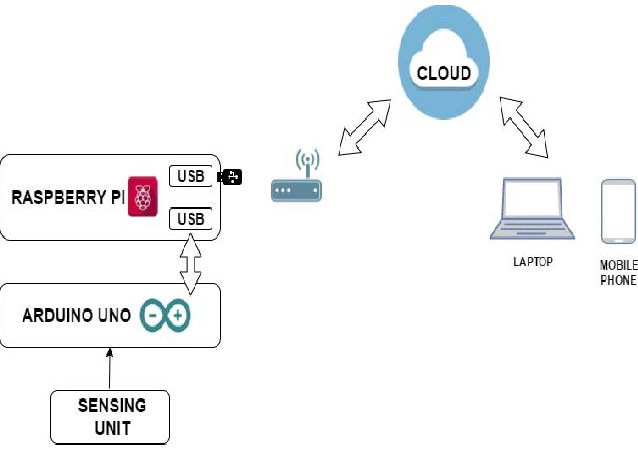
\includegraphics[scale=0.7]{figures/design}
\caption{\label{img31} Simplified diagram of Proposed System}
\end{figure}

Arduino Uno is a low-cost micro-controller board based on
ATMEGA-328P which can be easily interfaced with
Raspberry pi and has a very effective ADC. Since Raspberry
pi 4 has built in Wi-Fi adapter support therefore
Wi-Fi adapter is not used for providing the internet to the
complete system. The light weight protocol MQTT (Message
Queuing Telemetry transport). MQTT plays an important role
in establishing communication between the sensors and the
clients. The client can access the data that is being displayed
on the dashboard by using the device id but the client will be
not able to do any modification to the data received.

\subsection{Raspberry Pi}

Raspberry Pi is a single board computer. It has ARM
Cortex A8 CPU and 1 GB LPDDR4 RAM which makes it a faster and powerful than the previous available models. It has Broadcom
BCM2711, quad-core Cortex-A72 (ARM v8) processor which is running at 1.5 GHz but it can be overclocked. It has 2 × USB 3.0 ports and 2 × USB 2.0 ports, Standard 40-pin GPIO, 2 × micro HDMI ports (up to 4Kp60 supported), 2.4 GHz and 5.0 GHz IEEE 802.11b/g/n/ac wireless LAN, Bluetooth 5.0, 3.5 mm audio jack and
composite video, camera interface (CSI), the display interface
(DSI). It has a separate slot for Micro SD card slot which
is used for storing operating system as well as other software’s
and drivers needed. Raspberry Pi can support different
operating systems such as Raspbian, Windows 10, Ubuntu etc.
Raspbian operating system is used for implementation of
system. Node Red is a visual programming tool for IoT which
is very easy to use. Node Red has an inbuilt library consisting
of thousands of flows and nodes which enable the users to
connect all kind of devices and services. Once the flow is
made it can be deployed and data can be seen on the
dashboard.
\begin{figure}[!ht]
\centering
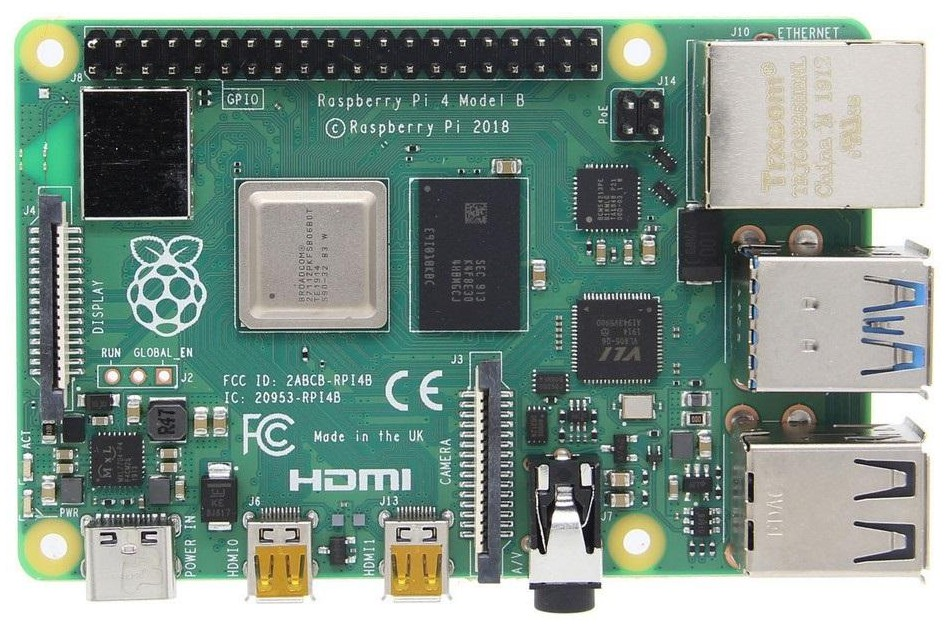
\includegraphics[width=\linewidth]{figures/raspberry.jpg}
\caption{\label{img32} Raspberry Pi 4}
\end{figure}

\begin{figure}[!ht]
\centering
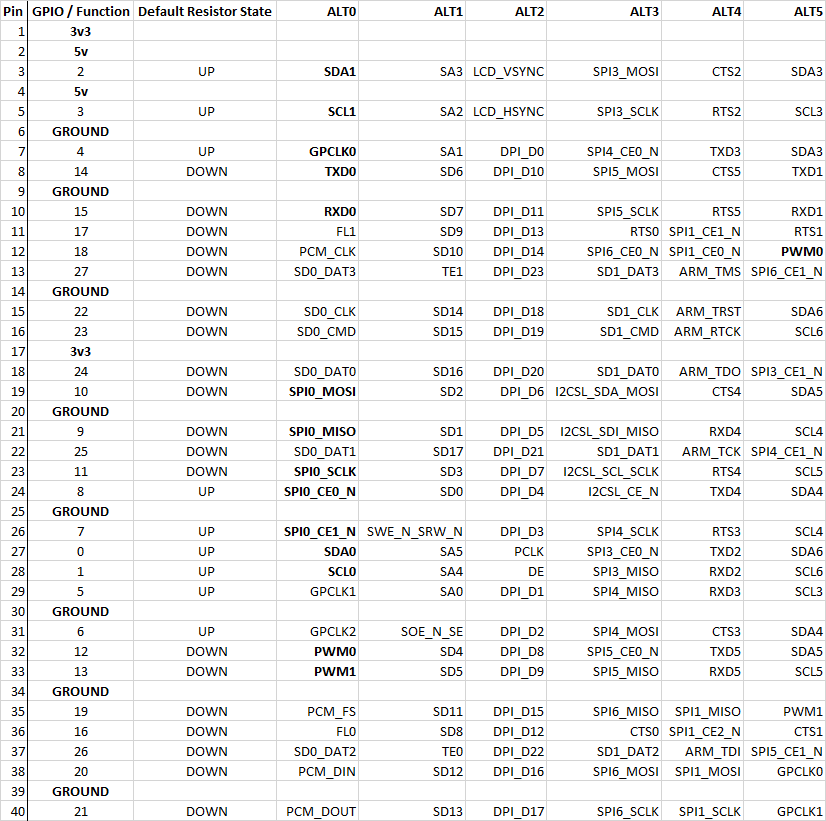
\includegraphics[width=\linewidth]{figures/raspberry-pindiagram.png}
\caption{\label{img33} Pin Diagram of Raspberry Pi 4}
\end{figure}

\begin{figure}[!ht]
\centering
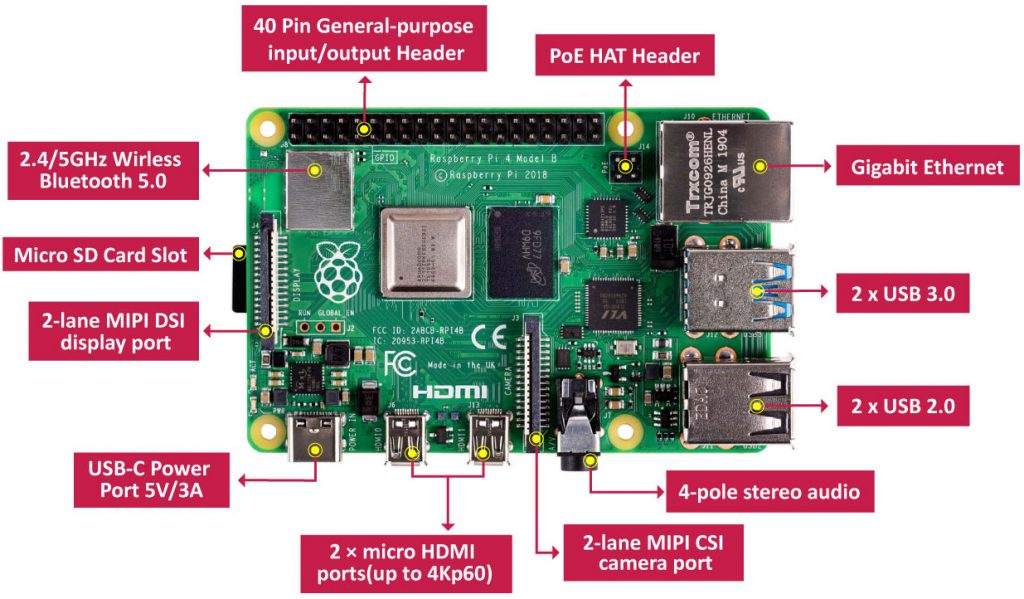
\includegraphics[width=\linewidth]{figures/Raspberry-Pi-pin.jpg}
\caption{\label{img34} Technical Configuration of Raspberry Pi 4}
\end{figure}


\subsection{Arduino UNO}

The Arduino UNO is an open-source microcontroller board based on the Microchip ATmega328P microcontroller and developed by Arduino.cc.The board is equipped with sets of digital and analog input/output (I/O) pins that may be interfaced to various expansion boards (shields) and other circuits. The board has 14 digital I/O pins (six capable of PWM output), 6 analog I/O pins, and is programmable with the Arduino IDE (Integrated Development Environment), via a type B USB cable. It can be powered by the USB cable or by an external 9-volt battery, though it accepts voltages between 7 and 20 volts. It is similar to the Arduino Nano and Leonardo

\begin{figure}[!ht]
\centering
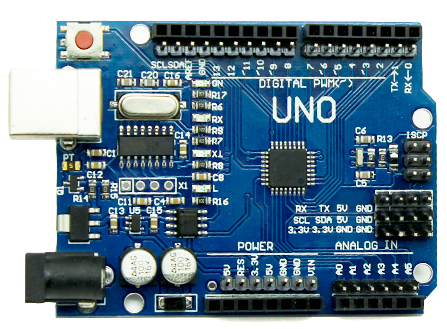
\includegraphics[scale=0.7]{figures/arduino-uno.png}
\caption{\label{img35} Arduino UNO}
\end{figure}

\begin{table}[!ht]
\centering
\begin{tabular}{ |p{5cm}|p{5cm}| }
\hline
\multicolumn{2}{|c|}{Technical specifications} \\
\hline
Microcontroller & ATmega328P\\
Operating Voltage & 5V\\
Input Voltage & 7-12V\\
Input Voltage (limit) & 7-20V\\
Digital I/O Pins & 14\\
PWM Digital I/O Pins & 6\\
Analog Input Pins & 6\\
DC Current per I/O pin & 20mA\\
Dc Current for 3.3V pin & 50mA\\
Flash Memory & 32 KB (ATmega328P)\\
SRAM & 2 KB (ATmega328P)\\
EEPROM & 1KB (ATmega328P)\\
Clock Speed & 16 MHz\\
Length & 68.6 mm\\
Width & 53.4 mm\\
\hline
\end{tabular}
\caption{\label{arduinopin}Arduino UNO Pin Diagram}
\end{table}


\begin{figure}[!ht]
\centering
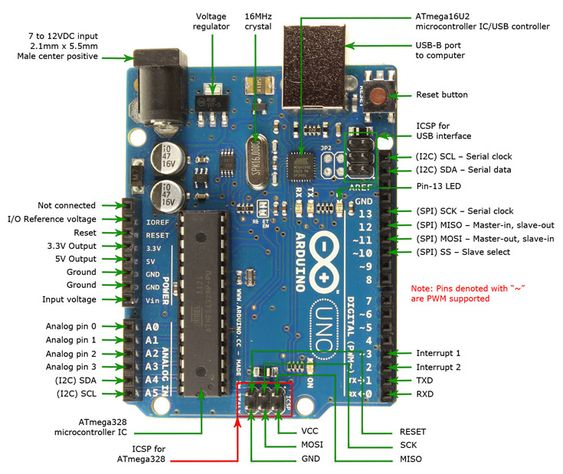
\includegraphics[scale=0.7]{figures/arduino-pin.jpg}
\caption{\label{img36} Technical Configuration of Arduino UNO}
\end{figure}

\subsection{Sensing Unit}

Sensing Unit comprises of five sensors for monitoring the
air pollution. Table 1 shows the technical specifications of the
three air quality sensors, Temperature, Humidity and pressure
sensors. DSM501A is a low-cost dust sensor module has a
very high sensitivity as it can even detect the fine particles
having the diameter greater than 1 micron. MQ9 is highly
sensitive to carbon monoxide / combustible gases. It has a
simple drive circuit and has a prolonged life. With the rise in
concentration of the gases in air, conductivity of the sensors
also increases. MQ135 has wide scope for detection of NH3,
alcohol, CO2, smoke, etc. with a very low response time.
DHT11 is a four-pin, resistive type having digital output
relative humidity and temperature sensor. BMP 180 is a low-
cost sensor used for monitoring barometric air pressure and
can also be used as an altimeter as the pressure changes with
the variations in altitude.

\begin{table}[!ht]
\centering
\begin{tabular}{ |p{4cm}|p{4cm}|p{4cm}|  }
\hline
\multicolumn{3}{|c|}{Sensors List} \\
\hline
Parameter & Operating Voltage & Measuring Range \\
\hline
Particulate Matter & 5 V  & 10 to 10000 ppm\\
Carbon Monoxide & 1.5 V  &10 to 10000 ppm\\
Carbon Dioxide & 5 V  & 10 to 10000 ppm\\
Temperature & 3.3 V  & -40 to +80 degree Celsius\\
Relative Humidity & 3.3 V & 0 to 100 \% RH\\
Pressure & 5 V & 300 to 1100 hPa\\
\hline
\end{tabular}
\caption{\label{sensorsvoltage}Sensors voltage range}
\end{table}


\subsection{Software Architecture}

It involves Node-Red and Integrated Development
Environment.

\subsubsection{Node-RED}

Node-RED is an easy to use, fundamental and an open
source programming tool for IoT applications. It is highly
used visual programming tool which help IoT developers to
integrate Hardware devices, APIs and online services in a very
interesting and creative manner. Built in Library of Node-Red
consist of thousands of flows and nodes that enable the user to
connect all kind of devices and services. Flows can be run at
the edge of network on the hardware like Raspberry pi or in
the cloud since node-red runtime includes node.js. Node-Red
provides a simple click mechanism to deploy the flows by the
IoT developers to a light weight runtime environment.

\subsubsection{Integrated Development Environment}

Arduino programs can be written in any programming
language that has a complier for a conversion of program code
into the binary code. IDE is platform independent acting as the
base for Arduino hardware. It is a very powerful for
programmers, project development professionals and
researchers to develop various Arduino projects employing
different kind of sensors. Arduino IDE is an open source
design/ software which has originated from the integrated
development environment for the languages processing and
wiring projects. As IDE is platform independent, it can run on
Windows, Linux based operating system as well as Mac OS. Some of the key features of IDE include a text console,
message area, toolbar for common functions. A program for
Arduino using IDE platform is known as sketch, languages
like C, C`++ are supported by Arduino IDE for programming.

\subsubsection{MQTT Protocol}

MQTT is extremely light weight connectivity protocol for
internet of things applications. It is designed for devices and
high latency, low bandwidth, unreliable network. Its
mainprinciple is to minimize device resource requirement and
network bandwidth. IANA reserved TCP/IP port 1883 for use
with MQTT over SSL. Unlike HTTP protocol it does not
MQTT is extremely light weight connectivity protocol for
internet of things applications. It is designed for devices and
high latency, low bandwidth, unreliable network. Its
mainprinciple is to minimize device resource requirement and
network bandwidth. IANA reserved TCP/IP port 1883 for use
with MQTT over SSL. Unlike HTTP protocol it does not
follow request/response architecture instead it follows
publish/subscribe architecture.

\section{Methodology}

Our sensor based Air quality monitoring system measuring
the ambient pollution is highly accurate, affordable, easy to
use. DSM501A is a PM sensor connected to digital pin 5 of
Arduino, DHT11, BMP180 are connected to the Digital pi3
and 4 of the Arduino where as MQ135 and MQ9 are
interfaced to analog pin 2 and 3 of Arduino. Arduino is
interfaced with Raspberry pi via a USB cable. Raspberry pi is
connected to internet with the help of Wi-Fi adapter and the
adapter is connected to Raspberry pi at USB port.

Initially operating system has to be installed into Raspberry
pi by downloading image from the Raspberry pi official
website. The file having .zip extension has to be unzipped to
retrieve .img file and write the image to the SD card.
As of November 2015, version of Raspbian Jessie,

As of November 2015, version of Raspbian Jessie, SD card
image is preinstalled with Node-RED and it is necessary to
upgrade it. When Pi boots up using the command “sudo
systemctl enable nodered.service” Node-RED starts running
automatically. In order to use cloud services of IBM, an
account is created at IBM Bluemix and at the same time
device is to be registered. Once the device is registered,
Bluemix IoT platform will acknowledge the user by providing
the Auth token which can be used for the communication of
data from device to Bluemix IoT platform.

The sensors are already connected to the Arduino board
and Raspberry pi is interfaced with Arduino. So, by deploying
a flow containing Serial in node to receive the data coming
from Serial port to raspberry pi, Serial in node is connected to
Watson IoT node for sending the data to the cloud. The data
can be seen on the dashboard of IBM Bluemix IOT platform
anywhere in the world, only requirement is that device should
be connected to internet.

\subsection{MQ-2 Gas Sensor}

The MQ-2 Gas sensor can detect or measure gasses like LPG, Alcohol, Propane, Hydrogen, CO and even methane. The module version of this sensor comes with a Digital Pin which makes this sensor to operate even without a microcontroller and that comes in handy when you are only trying to detect one particular gas. When it comes to measuring the gas in ppm the analog pin has to be used, the analog pin also TTL driven and works on 5V and hence can be used with most common microcontrollers.

\begin{figure}[!ht]
\centering
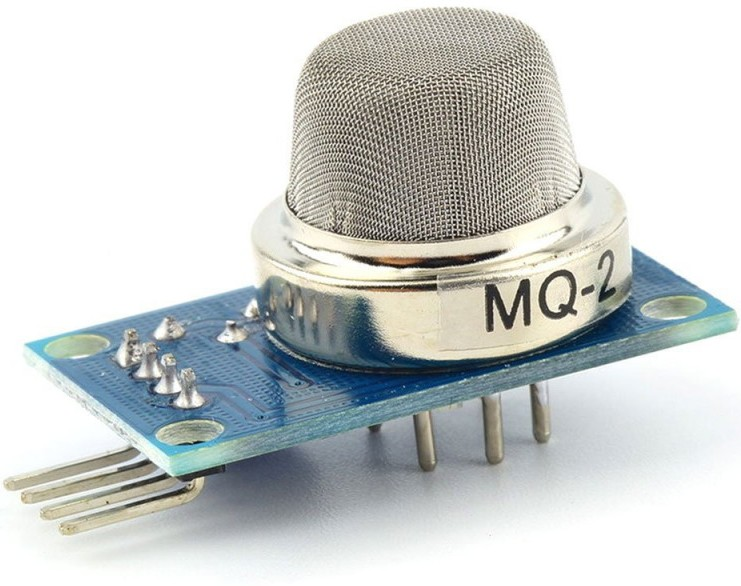
\includegraphics[width=12cm,height=7cm]{figures/mq-2.jpg}
\caption{\label{img37} MQ-2 Gas Sensor}
\end{figure}

\begin{table}[!ht]
\centering
\begin{tabular}{ |p{1cm}|p{2cm}|p{8cm}|  }
\hline
\multicolumn{3}{|c|}{Pin Configuration} \\
\hline
Pin No: & Pin Name: & Description \\
\hline
1 & Vcc  & This pin powers the module, typically the operating voltage is +5V\\
2 & Ground & Used to connect the module to system ground\\
3 & Digital Out & You can also use this sensor to get digital output from this pin, by setting a threshold value using the potentiometer\\
4 & Analog Out & This pin outputs 0-5V analog voltage based on the intensity of the gas \\
\hline
\end{tabular}
\caption{\label{mq-2pin}Pin Diagram of MQ-2 Sensor}
\end{table}


\begin{figure}[!ht]
\centering
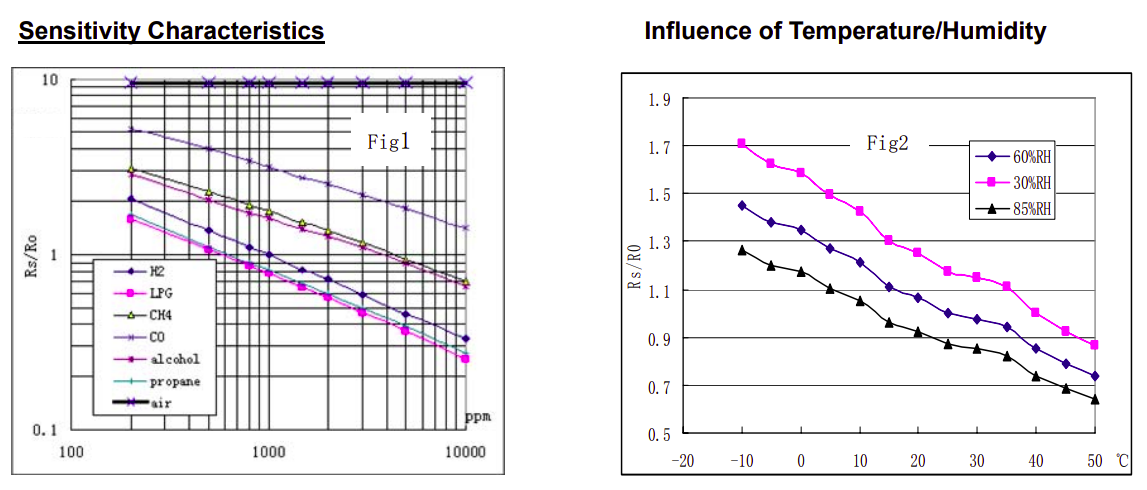
\includegraphics[width=\linewidth]{figures/mq2-datasheet.png}
\caption{\label{img38} MQ-2 Sensor Datasheet}
\end{figure}

\subsection{MQ-7 Carbon Monoxide Sensor}

The MQ-7 carbon monoxide sensor module allows for the sensing of CO concentrations in the air. This module can detect CO gas concentrations from anywhere between 20 and 2000ppm.

 It make detection by method of cycle high and low temperature, and detect CO when low temperature (heated by 1.5V). The sensor’s conductivity is more higher along with the gas concentration rising. When high temperature (heated by 5.0V), it cleans the other gases adsorbed under low temperature. The sensor is highly sensitive and has a quick response time. It uses analogue resistance as an output and is extremely easy to connect with any microcontroller.
 \begin{figure}[!ht]
\centering
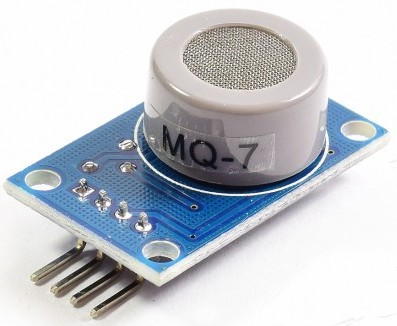
\includegraphics[width=12cm,height=7cm]{figures/mq-7.jpg}
\caption{\label{img39} MQ-7 Carbon Monoxide Sensor}
\end{figure} 
 
 \begin{table}[!ht]
\centering
\begin{tabular}{ |p{1cm}|p{2cm}|p{8cm}|  }
\hline
\multicolumn{3}{|c|}{Pin Configuration} \\
\hline
Pin No: & Pin Name: & Description \\
\hline
1 & Vcc  & This pin powers the module, typically the operating voltage is +5V\\
2 & Ground & Used to connect the module to system ground\\
3 & Digital Out & You can also use this sensor to get digital output from this pin, by setting a threshold value using the potentiometer\\
4 & Analog Out & This pin outputs 0-5V analog voltage based on the intensity of the gas \\
\hline
\end{tabular}
\caption{\label{mq-7pin}Pin Diagram of MQ-7 Sensor}
\end{table}
 
 
 
\begin{figure}[!ht]
\centering
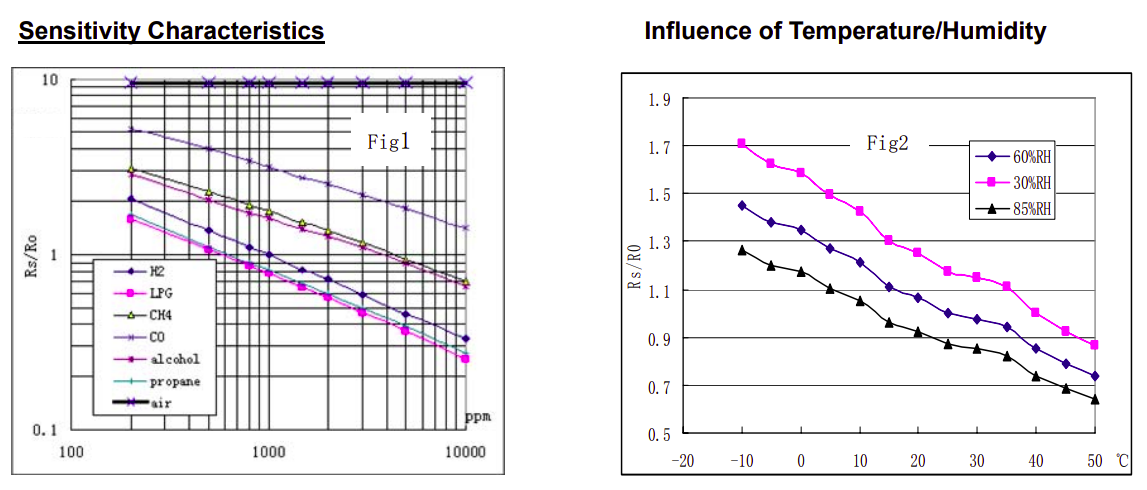
\includegraphics[width=\linewidth]{figures/mq7-datasheet.png}
\caption{\label{img310} MQ-7 Sensor Datasheet}
\end{figure}

\subsection{MQ-135 Air Quality Sensor }

The MQ-135 Gas sensors are used in air quality control equipments and are suitable for detecting or measuring of NH3, NOx, Alcohol, Benzene, Smoke, CO2. The MQ-135 sensor module comes with a Digital Pin which makes this sensor to operate even without a microcontroller and that comes in handy when you are only trying to detect one particular gas.  If you need to measure the gases in PPM the analog pin need to be used. The analog pin is TTL driven and works on 5V and so can be used with most common microcontrollers.

 \begin{figure}[!ht]
\centering
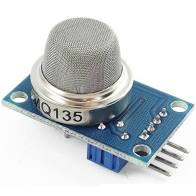
\includegraphics[width=12cm,height=10cm]{figures/mq-135.jpeg}
\caption{\label{img311} MQ-135 Air Quality Sensor}
\end{figure} 
 
 \begin{table}[!ht]
\centering
\begin{tabular}{ |p{1cm}|p{2cm}|p{8cm}|  }
\hline
\multicolumn{3}{|c|}{Pin Configuration} \\
\hline
Pin No: & Pin Name: & Description \\
\hline
1 & Vcc  & This pin powers the module, typically the operating voltage is +5V\\
2 & Ground & Used to connect the module to system ground\\
3 & Digital Out & You can also use this sensor to get digital output from this pin, by setting a threshold value using the potentiometer\\
4 & Analog Out & This pin outputs 0-5V analog voltage based on the intensity of the gas \\
\hline
\end{tabular}
\caption{\label{mq-135pin}Pin Diagram of MQ-135 Sensor}
\end{table}
 
 
 
\begin{figure}[!ht]
\centering
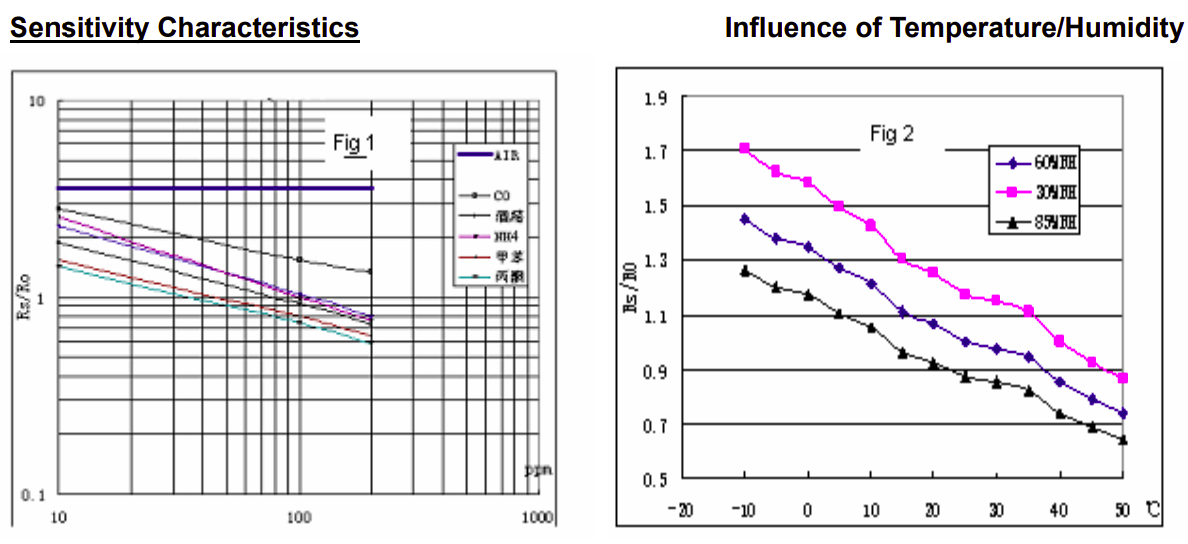
\includegraphics[width=\linewidth]{figures/mq135-datasheet.png}
\caption{\label{img312} MQ-135 Sensor Datasheet}
\end{figure}


\subsection{DHT-11 Temperature \& Humidity Sensor}

The DHT11 is a basic, ultra low-cost digital temperature and humidity sensor. It uses a capacitive humidity sensor and a thermistor to measure the surrounding air, and spits out a digital signal on the data pin (no analog input pins needed). Its fairly simple to use, but requires careful timing to grab data. The only real downside of this sensor is you can only get new data from it once every 2 seconds, so when using our library, sensor readings can be up to 2 seconds old.

\begin{figure}[!ht]
\centering
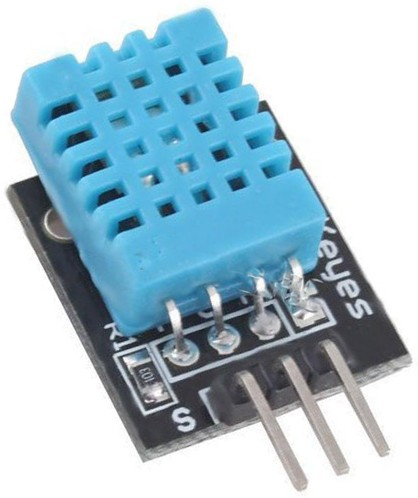
\includegraphics[width=12cm,height=10cm]{figures/dth11}
\caption{\label{img313} DHT-11 Temperature \& Humidity Sensor}
\end{figure}

\begin{table}[!ht]
\centering
\begin{tabular}{ |p{1cm}|p{2cm}|p{8cm}|  }
\hline
\multicolumn{3}{|c|}{Pin Configuration} \\
\hline
Pin No: & Pin Name: & Description \\
\hline
1 & Vcc  & Power supply 3.5V to 5.5V\\
2 & Data & Outputs both Temperature and Humidity through serial Data\\
3 & NC & No Connection and hence not used\\
4 & Ground & Connected to the ground of the circuits \\
\hline
\end{tabular}
\caption{\label{dht-11sensor}Pin Diagram of DHT-11 Sensor}
\end{table}
 
% Research~\cite{silber} in science and \index{technology} has played a vital role in improvising human life at great extent. With the development of instrumentation and computation facilities, research on frontier areas has gone manifold. The discussion on the frontier areas of research in inter- disciplinary subject has always yielded novel ideas and collaborative research. The aim of the conference is to provide a common platform to share and discuss the novel ideas, technologies and research findings to promote interdisciplinary research and to ignite young brains.


% \begin{table}[!ht]
% \centering
% \begin{tabular}{@{}p{10 cm}cccc@{}}\hline
% Research in science and technology & 1 & 2 & 3 & 5 \\
% Research in basic science& 1 & 2 & 3 & 5 \\
% Research in engineering sciences& 1 & 2 & 3 & 5 \\
% \hline
% \end{tabular}
% \caption{\label{data}Table caption 1}
% \end{table}

% Here is the description of Table~\ref{data}. Research in science and technology has played a vital role in improvising human life at great extent. With the development of instrumentation and computation facilities, research on frontier areas has gone manifold. 

% \begin{figure}[!ht]
% \centering
% \includegraphics[scale=0.9]{car1.png}
% \caption{\label{img5} Entity relation ship diagram}
% \end{figure}

% Description of Figure~\ref{img5}. .... 
% Research in science and technology has played a vital role in improvising human life at great extent. With the development of instrumentation and computation facilities, research on frontier areas has gone manifold. 



% \section{Summary}
% ............
 %Work done so far


\chapter{Implementation, Testing \& Result Analysis}\label{chap4}



\vspace*{40 ex}
%============================================================
\paragraph*{Outline:} This chapter presents the following:
\begin{enumerate}
\setlength{\itemsep}{-0.3em}
\item A brief of hardware implementation
\item A brief of software implementation
\item Testing of the project
\item Final result Analysis
\end{enumerate}
%============================================================

\newpage

\section{Hardware Implementation}

A hardware implementation means that the job is done using a physical device or electronic circuit as opposed to being done by a computer program. A hardware implementation often takes longer to create and that can make it more expensive. Hardware implementation is the building of the blocks of digital chip (either ASIC or FPGA) design and it relates them to the hardware description languages that are used in their creation

\subsection{Block Diagram}

\begin{figure}[!ht]
\centering
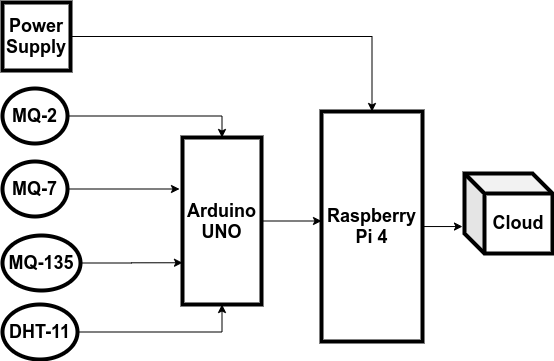
\includegraphics[width=\linewidth]{figures/arc-diagram.png}
\caption{\label{img41} An Architectural Diagram of the system.}
\end{figure}


\subsection{Flow Chart}

The flow of data should be cleared for every data processing unit and this study proposes a flow of data with simple and straight forward explanations which can see in figure~\ref{img42}. In this flow chart it's shown that every gas sensors and temperature have some threshold and if the value that are coming from sensors is less than given unit then it's counted as error and the value will be discarded.

\begin{figure}[!ht]
\centering
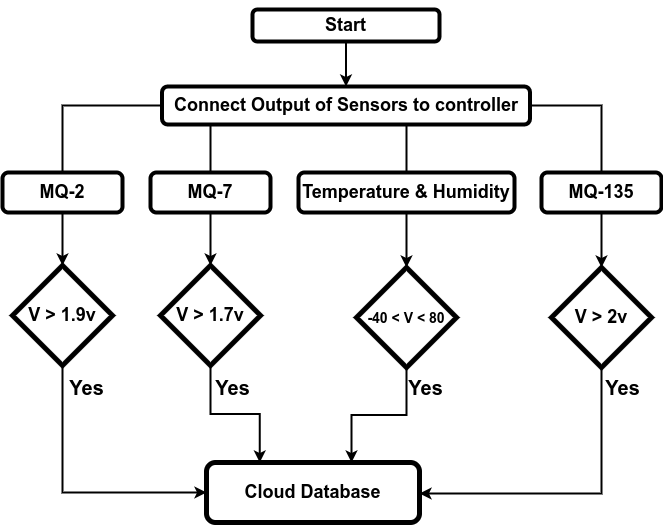
\includegraphics[width=\linewidth]{figures/flow-chart.png}
\caption{\label{img42} Flow of data from sensors to cloud database}
\end{figure}



\section{Software Implementation}

The software implementation stage involves the transformation of the software technical data package (TDP) into one or more fabricated, integrated, and tested software configuration items that are ready for software acceptance testing. The primary activities of software implementation include fabrication of software units to satisfy structural unit specifications, Assembly, integration, and testing of software components into a software configuration item.


\subsection{Hardware Data to cloud}

\subsubsection{Data Collection from MQ-2 sensor through Arduino Sketch}

\begin{lstlisting}[language=C, caption= Data calibration from MQ-2 Sensor]
const int inputPin = A0;
float R0;
int i = 1;
float LPGCurve[3] = {2.3,0.21,-0.47}; 
float COCurve[3] = {2.3,0.72,-0.34};
float SmokeCurve[3] = {2.3,0.53,-0.44}; 

void setup() {
  Serial.begin(9600);
  pinMode(inputPin, INPUT); 
  R0 = R0Calculate();
  delay(10000);
}

void loop() {
  float sensor_volt;
  float RS_gas; 
  float ratio; 

  float sensorValue = analogRead(inputPin); 
  
  sensor_volt = sensorValue*(5.0/1023.0);
  RS_gas = ((5.0*10.0)/sensor_volt)-10.0; 
  ratio = RS_gas/R0;  
  
  double  LPG = MQGetPercentage(ratio,LPGCurve);
  Serial.print(LPG);
  Serial.print(",");
  
  double  CO = MQGetPercentage(ratio,COCurve);
  Serial.print(CO);
  Serial.print(",");

  double  Smoke = MQGetPercentage(ratio,SmokeCurve);
  Serial.println(Smoke);
  delay(1000);
}

float R0Calculate(){
  float RS_air; 
  float R0;
  float sensorValue=0.0;
  float sensor_volt;
  
  for(int x = 0 ; x < 10000 ; x++) {
    sensorValue = sensorValue + analogRead(A0);
  }

  sensorValue = sensorValue/10000.0;
  sensor_volt = sensorValue*(5.0/1023.0); 
  RS_air = ((5.0*10.0)/sensor_volt)-10.0;
  R0 = RS_air/3.7;
  return R0;
}

double  MQGetPercentage(float rs_ro_ratio, float *pcurve) {
  return (pow(10,( ((log(rs_ro_ratio)-pcurve[1])/pcurve[2]) + pcurve[0])));
}

\end{lstlisting}


\subsubsection{Data calibration from Serial Port}
The most important part of calibration is watching the readings during the calibration process. It is easiest to calibrate the device in its default state (UART mode, with continuous readings enabled). Switching the device to I2C mode after calibration will not affect the stored calibration. If the device must be calibrated in I2C mode be sure to continuously request readings so you can see the output from the serial port, here we have initialized the baudrate 9600 that's best suited for Arduino UNO.

\begin{lstlisting}[language=Python, caption= Data calibration from Arduino Serial port]

import serial
from datetime import datetime
import firebase_admin
from firebase_admin import credentials
from firebase_admin import firestore

cred = credentials.Certificate("firebase-key.json")
firebase_admin.initialize_app(cred)
db = firestore.client()
col_ref = db.collection('coliberation')
ser = serial.Serial('/dev/ttyACM2',baudrate=9600,timeout=1)

while True:
    arduinoData = ser.readline().decode('ascii')
    sensorValue = arduinoData.split(',')

    if len(sensorValue)==3:
        LPG = float(sensorValue[0])
        _ = float(sensorValue[1])
        smoke = float(sensorValue[2])
        CO = float(sensorValue[3])
        airquality = float(sensorValue[4])
        CO2 = float(sensorValue[5])
        NH4 = float(sensorValue[6])
        temperature = float(sensorValue[7])
        humidity = float(sensorValue[8])
        data = {
            "time" : datetime.now(),
            "LPG" : LPG,
            "CO" : CO,
            "smoke" : smoke,
            "temperature" : temperature,
            "humidity" : humidity,
            "airquality" : airquality,
            "CO2" : CO2,
            "NH4" : NH4 
        }
        col_ref.add(data)
\end{lstlisting}

\subsection{ML Integration for Weather Forecast Prediction}

Weather forecasting is the application of science and technology to predict the conditions of the atmosphere for a given location and time. People have attempted to predict the weather informally for millennia and formally since the $19^{th}$ century. Weather forecasts are made by collecting quantitative data about the current state of the atmosphere at a given place and using meteorology to project how the atmosphere will change.

Once calculated by hand based mainly upon changes in barometric pressure, current weather conditions, and sky condition or cloud cover, weather forecasting now relies on computer-based models that take many atmospheric factors into account. Human input is still required to pick the best possible forecast model to base the forecast upon, which involves pattern recognition skills, teleconnections, knowledge of model performance, and knowledge of model biases. The inaccuracy of forecasting is due to the chaotic nature of the atmosphere, the massive computational power required to solve the equations that describe the atmosphere, the error involved in measuring the initial conditions, and an incomplete understanding of atmospheric processes. Hence, forecasts become less accurate as the difference between current time and the time for which the forecast is being made (the range of the forecast) increases. 

There is a vast variety of end uses to weather forecasts. Weather warnings are important forecasts because they are used to protect life and property. Forecasts based on temperature and precipitation are important to agriculture, and therefore to traders within commodity markets. Temperature forecasts are used by utility companies to estimate demand over coming days.

\subsubsection{Dataset and Data Preprocessing}

This dataset contains 6 different features such as air temperature, atmospheric pressure, humidity, Windspeed and WindDirection. These were collected every 1 hour, beginning on 29 May 2020 to ending on 12 June 2020. This section of the dataset was collected from meteoblue(https://www.meteoblue.com/en/weather) that consists of 328 time series data. 

It is important to scale features before training a neural network. Standardization is a common way of doing this scaling by subtracting the mean and dividing by the standard deviation of each feature. 

The data preprocessing is being done by standard method,
Suppose there are n number of data points present in dataset and their values are $X_1, X_2, X_3, X_4, X_5 ....., X_n$ and $X_{mean}$ is a mean of all data points and $X_{dev}$ is a standard deviation of all data points and their calculation is following 

\[ X_{mean} = \dfrac{X_1 + X_2 + X_3 + X_4 + X_5 + ....... + X_n }{n} \]
\[X_{dev}^{2} = \sqrt{ ( X_1 -X_{mean} + X_2 -X_{mean} + X_3 -X_{mean} + .... + X_n -X_{mean} )^2}\]
\[ X_i = \dfrac{X_i - X_{mean}}{X_{dev}} i = 1, 2, 3, ..., n\]

\subsubsection{Model}
This study use LSTM model which is a deep
learning model proposed by Schmidhuber (Hochreiter
and Schmidhuber, 1997). The model has been
successfully used in many research fields such as,
large scale image classification (Real et al., 2017),
video classification (Yoo, 2017), natural language
processing (Elkaref and Bohnet, 2017), anomaly
detection (Luo et al., 2017; Lee et al., 2018). LSTM
was used as a foundation for weather forecasting
model because of several reasons that are the
model ability to solve long lag relationship in time
series data (2) the model ability to address vanisihing
gradient problems that occur in the training deep
structure neural networks (Gers et al, 2000). 

LSTM is a recurrence Neural Network that first
introduced by (Hochreiter and Schmidhuber, 1997) as a
specific Recurrent Neural Network (RNN) architecture that was designed to model temporal sequences. Better
than the conventional RNN, LTSTM is able to sort error
backflow problem so that this algorithm only use the
error feedback that can make more accurate prediction
whereas all unsupported feedback are removed. This
algorithm has sorting capability due to LSTM contains
special units called memory blocks in the recurrent
hidden layer. The LSTM overcome the weakness in
conventional RNN that show backpropagation algorithm
in RNNs cause error signals that flows backward in time
tend to explode or diminish; therefore, the temporal
evolution of the backpropagated error exponentially
depends on the size of the weight. In other words, the
strength of LSTM is special units called memory blocks
in the recurrent hidden layer. 

As we know that any Machine Learning(ML) or Deep Learning(DL) can only predict one feature although we can provide multiple features as input and based on those input features and also depends upon past history any model predict future data but the weather forecast needs multiple features like temperature, pressure, humidity, wind-speed and many more that is why this this project really needs more than one model to predict multiple features.

This entire modelling part is divided into three sub sections

\begin{itemize}
\item section 1: The prediction of temperature with univariate feature and timestamp as an input feature for prediction.

\item section 2: The prediction of humidity with univariate feature and timestamp as an input feature for prediction.

\item section 3: The prediction of pressure with univariate feature and timestamp as an input feature for prediction.
\end{itemize}

\subsubsection{Flow Chart}
The flow of data should be cleared for every data processing unit and this study proposes a flow of data with simple and straight forward explanations which can see figure~\ref{img43}.

\begin{figure}[!ht]
\centering
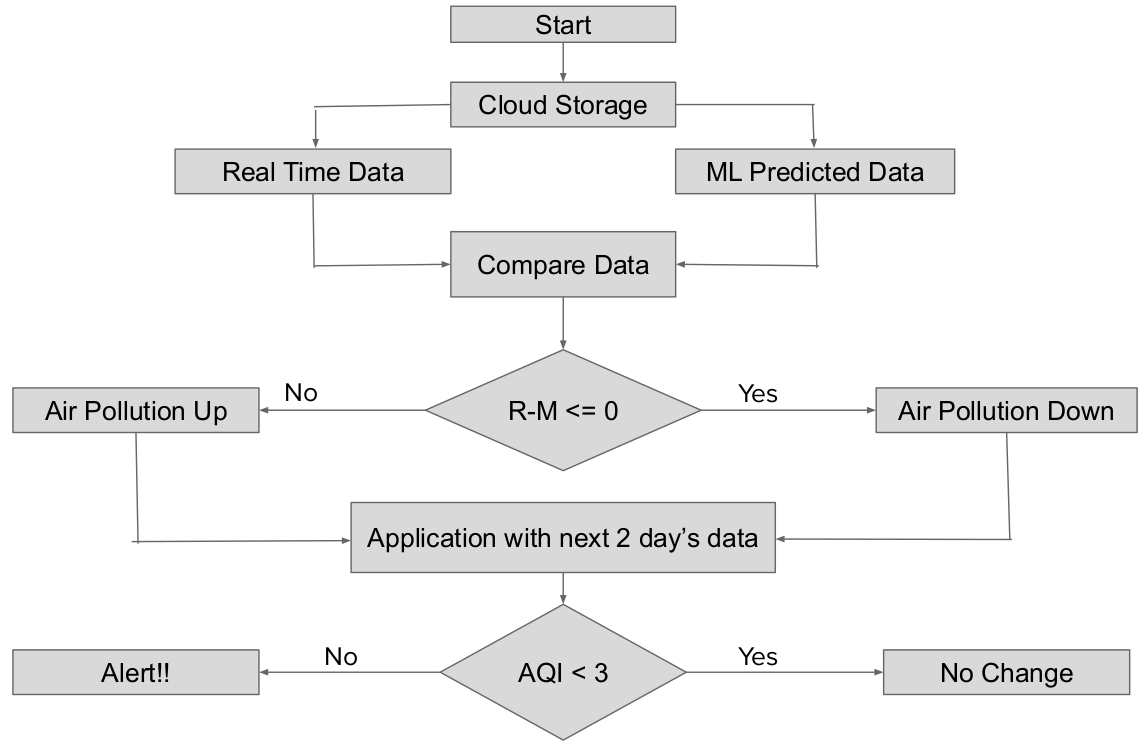
\includegraphics[width=\linewidth]{figures/ml-flow-chart.png}
\caption{\label{img43} flow of real time data with predicted data}
\end{figure}

\subsubsection{Logic Implementation}

\begin{figure}[!ht]
\centering
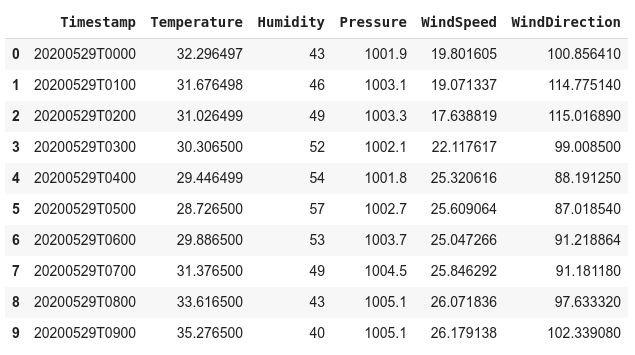
\includegraphics[width=\linewidth]{figures/sample-data.png}
\caption{\label{img44} sample of every an hour data}
\end{figure}

As you can see in figure~\ref{img44}, an observation is recorded every 1 hours. This means that, for a single hour, you will have only 1 observations. Similarly, a single day will contain 24 (1x24) observations.

Given a specific time, let's say you want to predict the temperature 6 hours in the future. In order to make this prediction, you choose to use 5 days of observations. Thus, you would create a window containing the last 120(5x24) observations to train the model. Many such configurations are possible, making this dataset a good one to experiment with.

The function below returns the above described windows of time for the model to train on. The parameter history\_size is the size of the past window of information. The target\_size is how far in the future does the model need to learn to predict. The target\_size is the label that needs to be predicted.

\begin{lstlisting}[language=Python, caption= A function to return windows of time followed by history\_size ]
def univariate_data(dataset, start_index, end_index, history_size, target_size):
  data = []
  labels = []
  start_index = start_index + history_size
  if end_index is None:
    end_index = len(dataset) - target_size
  for i in range(start_index, end_index):
    indices = range(i-history_size, i)
    # Reshape data from (history_size,) to (history_size, 1)
    data.append(np.reshape(dataset[indices], (history_size, 1)))
    labels.append(dataset[i+target_size])
  return np.array(data), np.array(labels)
\end{lstlisting}

It is important to scale features before training a neural network. Standardization is a common way of doing this scaling by subtracting the mean and dividing by the standard deviation of each feature.You could also use a tf.keras.utils.normalize method that rescales the values into a range of [0,1]. Note: The mean and standard deviation should only be computed using the training data.

\begin{lstlisting}[language=Python, caption= Scaling the feature by standard method]
uni_train_mean = uni_data[:TRAIN_SPLIT].mean()
uni_train_std = uni_data[:TRAIN_SPLIT].std()
uni_data = (uni_data-uni_train_mean)/uni_train_std
\end{lstlisting}

Let's now create the data for the univariate model. For our first model, the model will be given the last 20 recorded temperature observations, and needs to learn to predict the temperature at the next time step.

\begin{lstlisting}[language=Python, caption= Splitting data into training-set and validation-set]
univariate_past_history = 20
univariate_future_target = 0

x_train_uni, y_train_uni = univariate_data(uni_data, 0, TRAIN_SPLIT,
                                           univariate_past_history,
                                           univariate_future_target)
x_val_uni, y_val_uni = univariate_data(uni_data, TRAIN_SPLIT, None,
                                       univariate_past_history,
                                       univariate_future_target)
\end{lstlisting}

due to less availability of data our long short term memory(LSTM) model is simple and with the less number of happen layers and dense layers because adding more layers may lead to overfit or underfit this is something which we don't want. There summary of our model can see in figure~\ref{img45}

\begin{lstlisting}[language=Python, caption= Creating a LSTM model with their summary]
simple_lstm_model = tf.keras.models.Sequential([
    tf.keras.layers.LSTM(8, input_shape=x_train_uni.shape[-2:]),
    tf.keras.layers.Dense(1)
])

simple_lstm_model.compile(optimizer='adam', loss='mae')
simple_lstm_model.summary()

\end{lstlisting}

\begin{figure}[!ht]
\centering
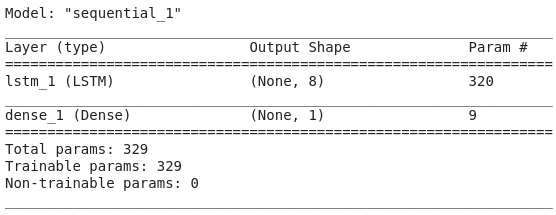
\includegraphics[width=\linewidth]{figures/model-summary.png}
\caption{\label{img45} Summary of simple long short term memory model}
\end{figure}

\subsection{Flutter Application}
Flutter is an open-source UI software development kit created by Google. It is used to develop applications for Android, iOS, Windows, Mac, Linux, Google Fuchsia and the web from a single codebase.

The first version of Flutter was known as codename "Sky" and ran on the Android operating system. It was unveiled at the 2015 Dart developer summit, with the stated intent of being able to render consistently at 120 frames per second.

Flutter apps are written in the Dart language and make use of many of the language's more advanced features.Flutter runs in the Dart virtual machine which features a just-in-time execution engine. While writing and debugging an app, Flutter uses Just In Time compilation, allowing for "hot reload", with which modifications to source files can be injected into a running application. Flutter extends this with support for stateful hot reload, where in most cases changes to source code can be reflected immediately in the running app without requiring a restart or any loss of state.Release versions of Flutter apps are compiled with ahead-of-time (AOT) compilation on both Android and iOS, making Flutter's high performance on mobile devices possible.

\subsubsection{Fetching data from cloud}

StreamBuilder is a Widget that can convert a stream of user defined objects, to widgets. This takes two arguments stream and builder, that can convert the elements of the stream to widgets
Suppose, you have a Stream, that updates if there is any UI update (may be from user interaction, or may be resulted from network updates). If your “main” widget, includes a StreamBuilder, which listens to the stream, it can act as the element in charge of translating your states to views.

\begin{lstlisting}[language=java, caption = Getting data from cloud database to flutter UI]
StreamBuilder<QuerySnapshot>(
        stream: _database.snapshots(),
        builder: (BuildContext context, AsyncSnapshot<QuerySnapshot> snapshot) {
          if (snapshot.hasError)
            return new Text('Error: ${snapshot.error}');
          switch (snapshot.connectionState) {
            case ConnectionState.waiting: return new Text('Loading...');
            default:
              return ListView.builder(
                  shrinkWrap: true,
                  itemCount: snapshot.data.documents.length,
                  itemBuilder: (BuildContext context, int index) {
                    double temperature = snapshot.data.documents[index]['temperature'];
                    double humidity = snapshot.data.documents[index]['humidity'];
                    dynamic time = snapshot.data.documents[index]['time'].toDate();
                    return Card(
                        color: Colors.deepOrange[400],
                        elevation: 10,
                        shape: RoundedRectangleBorder(
                          borderRadius: BorderRadius.circular(15.0),
                        ),
                        child: new Row(
                          mainAxisAlignment: MainAxisAlignment.spaceEvenly,
                          mainAxisSize: MainAxisSize.max,
                          children: <Widget>[
                            layout("Temperature",temperature, "Time", time, "Humidity", humidity),
                          ],
                        )
                    );
                  });
          }
        },
      ),

\end{lstlisting}

\subsubsection{Fetching data from ML API}
Long-running tasks are common in mobile apps. The way this is handled in Flutter / Dart is by using a Future. A Future allows you to run work asynchronously to free up any other threads that should not be blocked. Like the UI thread.

A future is defined exactly like a function in dart, but instead of void you use Future. If you want to return a value from the Future then you pass it a type.

\begin{lstlisting}[language=java, caption = Getting data from ML API to flutter UI]
Future<dynamic> getPrediction(year,month,day,hour,minute,humidity) async{
    final url = '$baseUrl/date/?name=$year,$month,$day,$hour,$minute,$humidity';
    print('fetching $url');
    final res = await httpClient.get(url);
    if (res.statusCode != 200) {
      throw HTTPException(res.statusCode, "unable to fetch weather data");
    }
    final predictionData = json.decode(res.body);
    return predictionData;
  }
\end{lstlisting}

\subsubsection{Fetching data from Weather API}

Future operations are the operations which take time to perform and return the result later. To handle this problem, we use Asynchronous functions. Asynchronous operations let your program continue other operations while the current operation is being performed. Dart uses Future objects (futures) to represent the results of asynchronous operations. To handle these operations, we can use Async/await, but it is not possible to integrate async and await on widgets. So it is quite tricky to handle futures in widgets. To solve this problem flutter provided a widget called Future Builder.

\begin{lstlisting}[language=java, caption = Getting data from Weather API to flutter UI]
FutureBuilder(
        future: getData(DateTime.now(), humidity),
        builder: (context, snapshot){
              dynamic keys = snapshot.data.keys.toList();
              DateTime time = new DateTime.now();
              return ListView.builder(
                itemCount: snapshot.data.length,
                itemBuilder: (BuildContext context, int index) {
                  final temp = snapshot.data[keys[index]].round();
                  var newtime = time.add(new Duration(seconds: 60*index));
                  var now = timePormat(newtime.year, newtime.month, newtime.day, newtime.hour,newtime.minute);
                  return Card(
                      color: Colors.deepOrange[400],
                      elevation: 10,
                      shape: RoundedRectangleBorder(
                        borderRadius: BorderRadius.circular(15.0),
                      ),
                      child: Text('$temp $now'),
                      )
                  );
                },
              );
          }
        }
    );
\end{lstlisting}
\section{Testing \& Result Analysis}

From a proper analysis of positive points and constraints on the component, it can be safely concluded that the product is a highly efficient GUI based component and with accurate weather forecasting system. This system is working properly and meeting to most of the user requirements. This component can be easily plugged in many other systems.

The aim of the proposed system testing process was to determine all defects in the project .The program was subjected to a set of test inputs and various observations were made and based on these observations it will be decided whether the program behaves as expected or not.

Testing and result analysis of this proposed is done in following three parts.
\begin{itemize}
\item Gas and Temperature sensors testing
\item Forecasting Models testing
\item Flutter application testing
\end{itemize}

\subsection{Gas and Temperature Sensors}
Data calibration of this proposed system is done using gas and temperature sensors such as MQ-2 gas sensor, MQ-7 carbon monoxide sensor, MQ-135 air quality sensor and DHT-11 temperature and humidity sensor and the working of these sensors with their datasheet is already explained in section 3.2, there are following parameters are tested in above mention sensors.
\begin{itemize}
\item Temperature
\item Humidity
\item Air Quality
\item Carbon Monoxide Gas
\item Carbon Dioxide Gas
\item Ammonium Gas
\item LPG Gas
\item Smoke
\end{itemize}


\subsection{Temperature}
Temperature is a physical property of matter that quantitatively expresses hot and cold. It is the manifestation of thermal energy, present in all matter, which is the source of the occurrence of heat, a flow of energy, when a body is in contact with another that is colder.
DHT-11(temperature and humidity) sensor is used to calibrate temperature.
\begin{figure}[!ht]
\centering
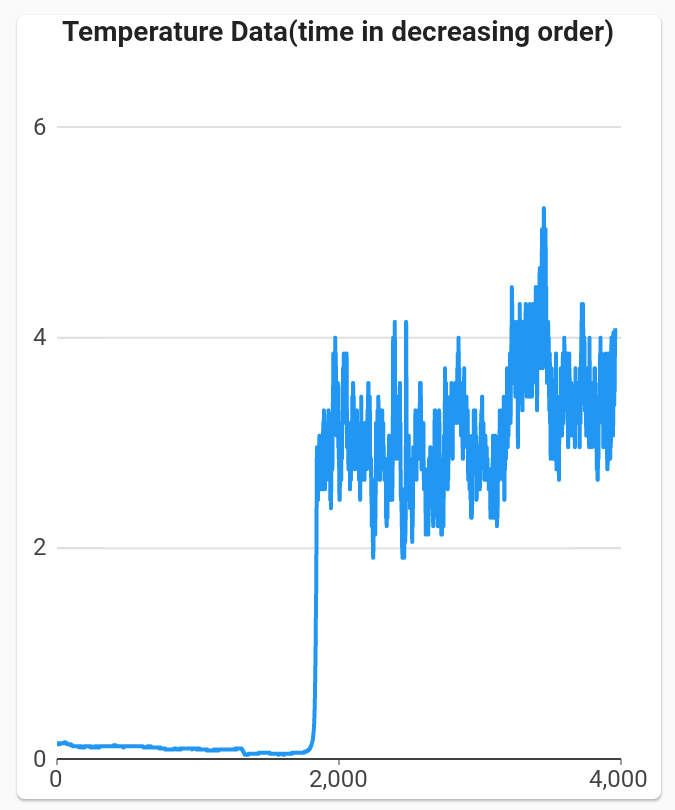
\includegraphics[width=\linewidth,height=8cm]{figures/temp.png}
\caption{\label{img46} Temperature variation with respect to time}
\end{figure}

\subsection{Humidity}
Humidity is the concentration of water vapor present in the air. Water vapor, the gaseous state of water, is generally invisible to the human eye. Humidity indicates the likelihood for precipitation, dew, or fog to be present. The amount of water vapor needed to achieve saturation increases as the temperature increases. As the temperature of a parcel of air decreases it will eventually reach the saturation point without adding or losing water mass. The amount of water vapor contained within a parcel of air can vary significantly. DHT-11(temperature and humidity) sensor is used to calibrate humidity.

\begin{figure}[!ht]
\centering
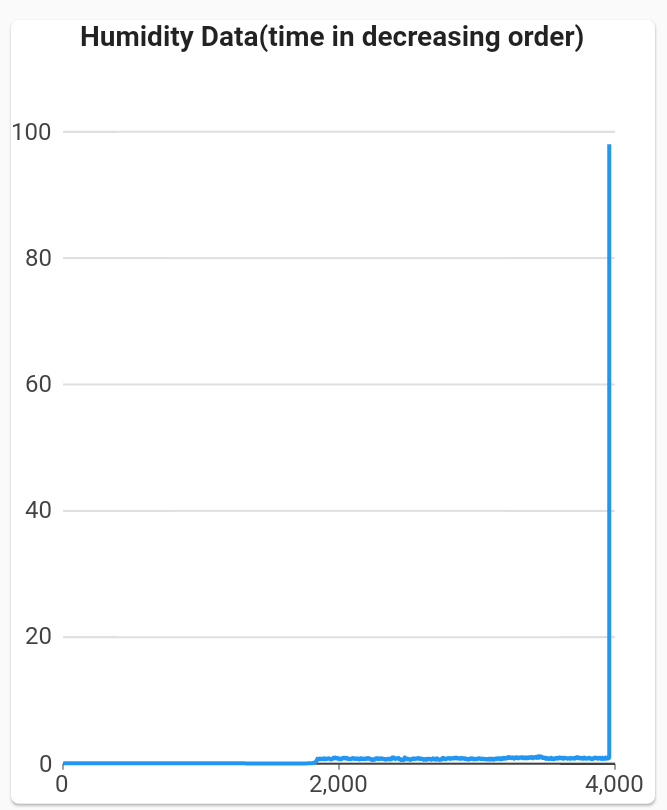
\includegraphics[width=\linewidth,height=8cm]{figures/humidity.png}
\caption{\label{img47} Humidity variation with respect to time}
\end{figure}

\subsection{Air Quality}
To measure air quality air quality index (AQI) unit is used.
An air quality index (AQI) is used by government agencies to communicate to the public how polluted the air currently is or how polluted it is forecast to become. Public health risks increase as the AQI rises. Different countries have their own air quality indices, corresponding to different national air quality standards. MQ-135 sensor is used to calibrate air quality.
\begin{figure}[!ht]
\centering
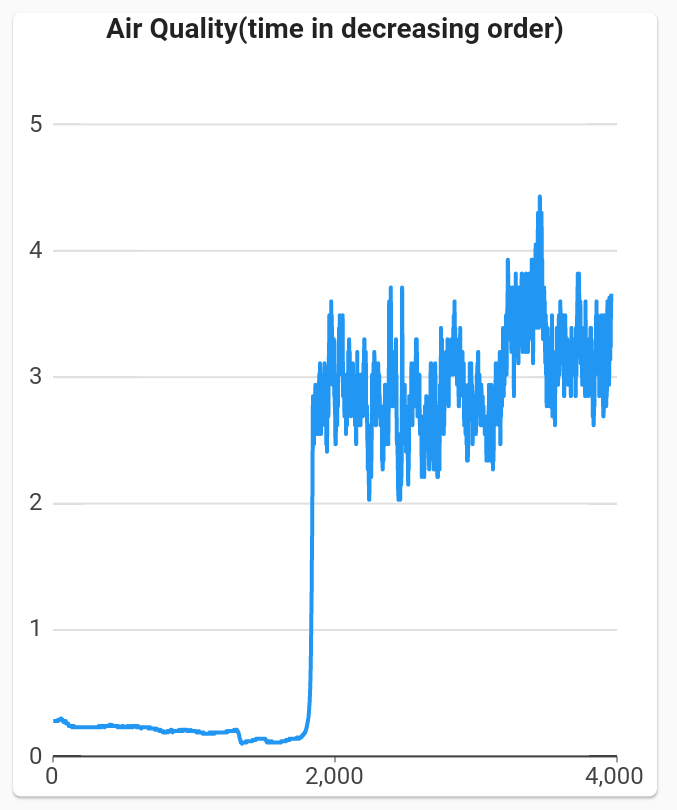
\includegraphics[width=\linewidth,height=8cm]{figures/airquality.png}
\caption{\label{img48} Air Quality variation with respect to time}
\end{figure}

\subsection{Carbon Monoxide Gas}
Carbon monoxide(CO) is a colorless, odorless, and tasteless flammable gas that is slightly less dense than air. It is toxic to animals that use hemoglobin as an oxygen carrier (both invertebrate and vertebrate) when encountered in concentrations above about 35 ppm, although it is also produced in normal animal metabolism in low quantities, and is thought to have some normal biological functions. In the atmosphere, it is spatially variable and short-lived, having a role in the formation of ground-level ozone. MQ-7 sensor is used to calibrate Carbon monoxide(CO).

\begin{figure}[!ht]
\centering
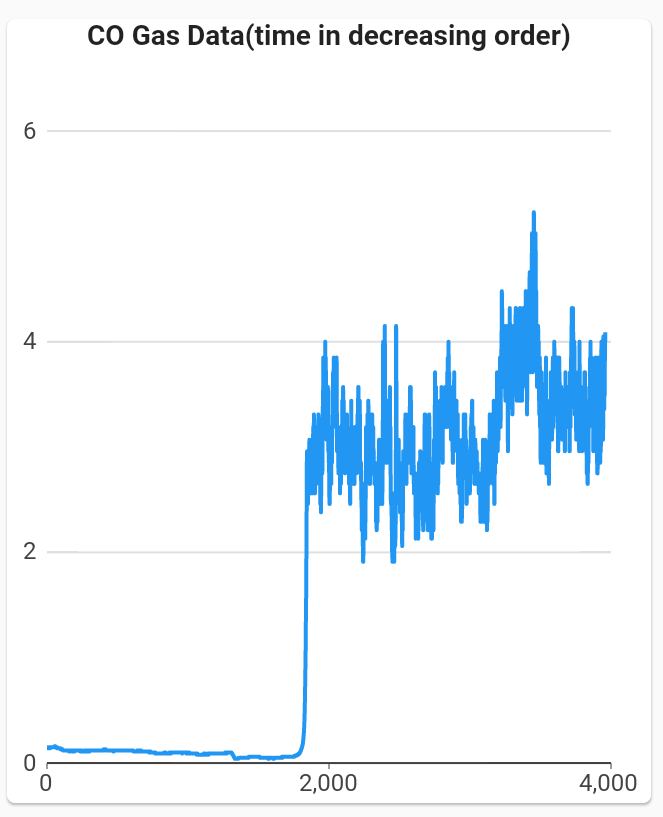
\includegraphics[width=\linewidth,height=8cm]{figures/CO.png}
\caption{\label{img49} Carbon Monoxide(CO) variation with respect to time}
\end{figure}

\subsection{Carbon Dioxide Gas}
Carbon dioxide is a colorless gas with a density about 60\% higher than that of dry air. Carbon dioxide consists of a carbon atom covalently double bonded to two oxygen atoms. It occurs naturally in Earth's atmosphere as a trace gas. The current concentration is about 0.04\% (412 ppm) by volume, having risen from pre-industrial levels of 280 ppm.[8] Natural sources include volcanoes, hot springs and geysers, and it is freed from carbonate rocks by dissolution in water and acids. Because carbon dioxide is soluble in water, it occurs naturally in groundwater, rivers and lakes, ice caps, glaciers and seawater.  MQ-2 sensor is used to calibrate Carbon Dioxide($CO_{2}$).
\begin{figure}[!ht]
\centering
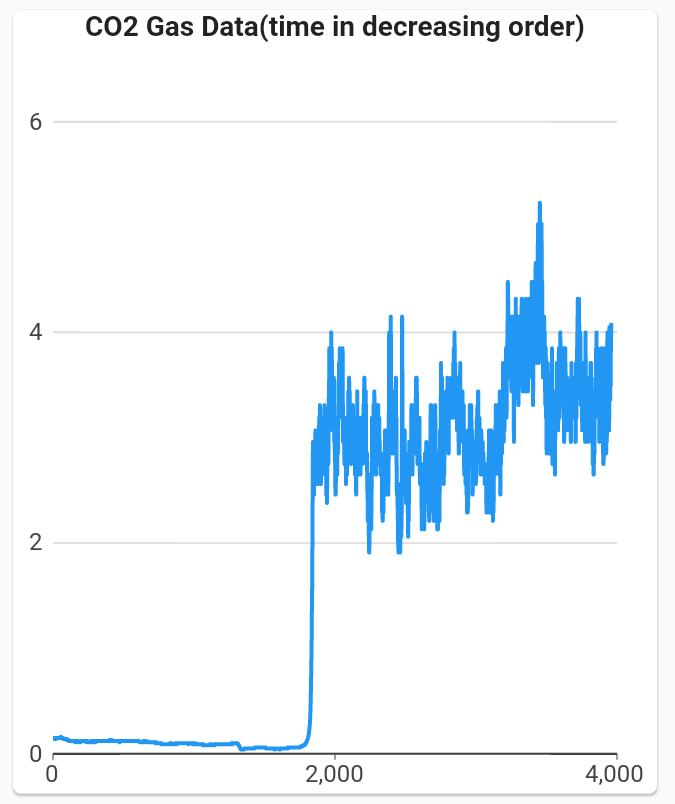
\includegraphics[width=\linewidth,height=8cm]{figures/CO2.png}
\caption{\label{img410} Carbon Dioxide($CO_{2}$) variation with respect to time}
\end{figure}

\subsection{Ammonium Gas}
Ammonia is a compound of nitrogen and hydrogen with the formula NH3. A stable binary hydride, and the simplest pnictogen hydride, ammonia is a colourless gas with a characteristic pungent smell. It is a common nitrogenous waste, particularly among aquatic organisms, and it contributes significantly to the nutritional needs of terrestrial organisms by serving as a precursor to food and fertilizers. Ammonia, either directly or indirectly, is also a building block for the synthesis of many pharmaceutical products and is used in many commercial cleaning products. It is mainly collected by downward displacement of both air and water.
\begin{figure}[!ht]
\centering
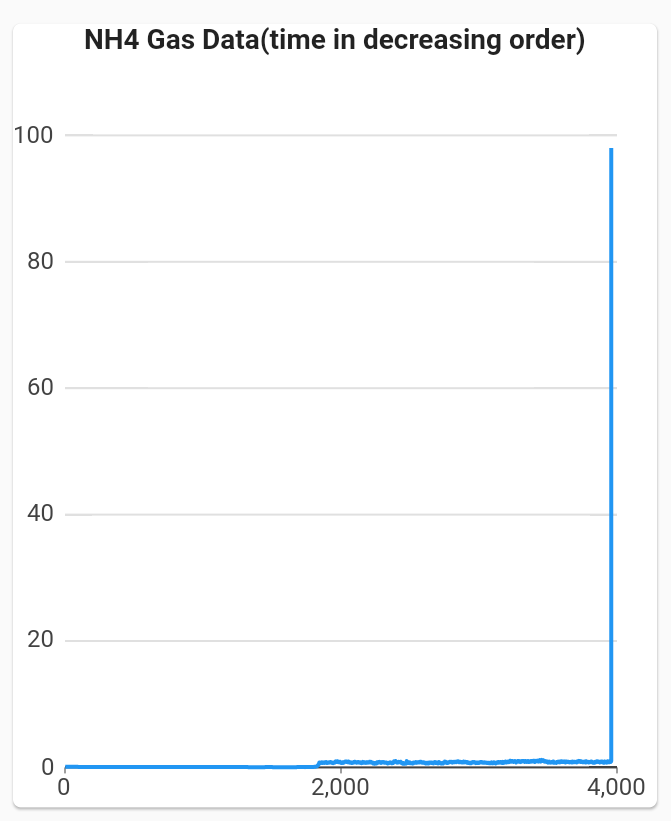
\includegraphics[width=\linewidth,height=8cm]{figures/NH4.png}
\caption{\label{img411} Ammonium($NH_{4}$) variation with respect to time}
\end{figure}

\subsection{LPG Gas}
Liquefied petroleum gas or liquid petroleum gas (LPG or LP gas), is a flammable mixture of hydrocarbon gases used as fuel in heating appliances, cooking equipment, and vehicles.

It is increasingly used as an aerosol propellant and a refrigerant, replacing chlorofluorocarbons in an effort to reduce damage to the ozone layer. When specifically used as a vehicle fuel it is often referred to as autogas.
\begin{figure}[!ht]
\centering
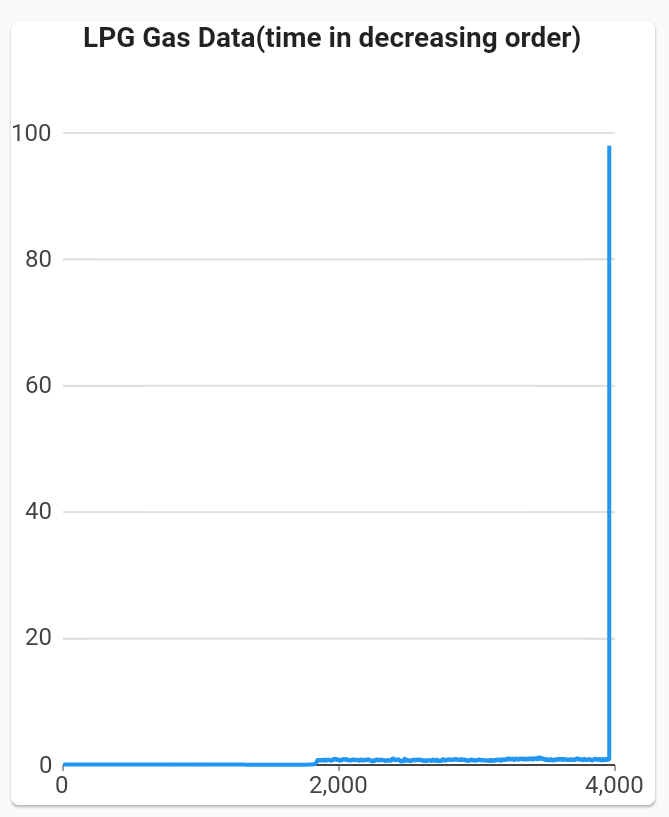
\includegraphics[width=\linewidth,height=8cm]{figures/LPG.png}
\caption{\label{img412} LPG variation with respect to time}
\end{figure}

\subsection{Smoke}
Smoke is a collection of airborne particulates and gases[1] emitted when a material undergoes combustion or pyrolysis, together with the quantity of air that is entrained or otherwise mixed into the mass. It is commonly an unwanted by-product of fires (including stoves, candles, internal combustion engines, oil lamps, and fireplaces), but may also be used for pest control (fumigation), communication (smoke signals), defensive and offensive capabilities in the military (smoke screen), cooking, or smoking (tobacco, cannabis, etc.). It is used in rituals where incense, sage, or resin is burned to produce a smell for spiritual or magical purposes. It can also be a flavoring agent and preservative for various foodstuffs.
\begin{figure}[!ht]
\centering
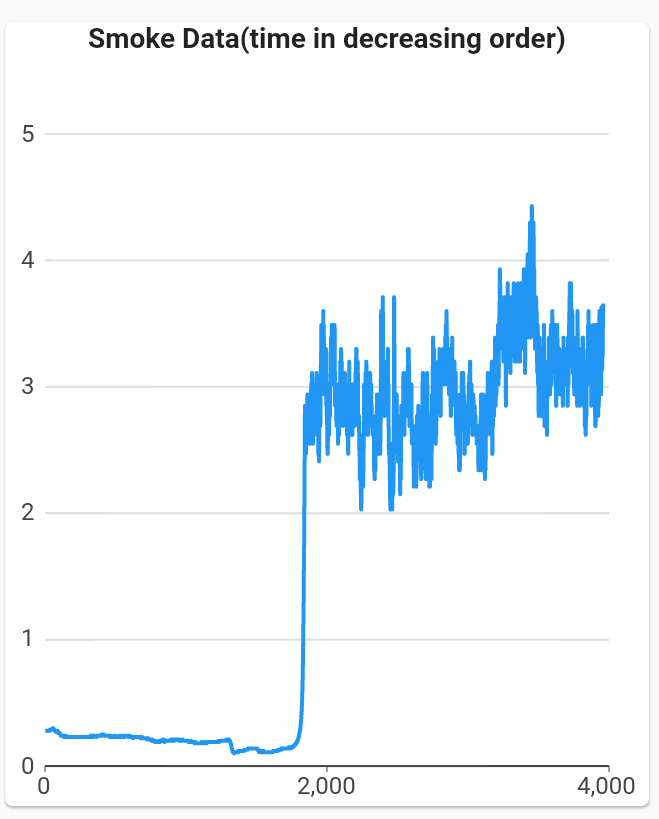
\includegraphics[width=\linewidth,height=8cm]{figures/smoke.png}
\caption{\label{img413} Smoke variation with respect to time}
\end{figure}


\subsection{Forecasting Models}
For the predicting weather forecast three different models are made. Model-1 is responsible for predicting temperature, model-2 is responsible for predicting humidity and model-3 is responsible for predicting pressure. The dataset and preprocesing part is explained in section 4.2.2.1, modelling part is explained in section 4.2.2.2 and the implementation of logic is explained in section 4.2.2.4, the table 4.1 summarizing models with their accuracy.

\begin{table}[!ht]
\centering
\begin{tabular}{ |p{2cm}|p{2cm}|p{2cm}|p{2cm}|p{2cm}| }
\hline
\multicolumn{5}{|c|}{Weather Forecasting Models} \\
\hline
Model&Feature&Training Data&Testing Data&Accuracy \\
\hline
Model-1&Temperature&80\%&20\%&73\%\\
Model-2 &Humidity&80\%&20\%&73\%\\
Model-3 &Pressure&80\%&20\%&73\%\\
\hline
\end{tabular}
\caption{\label{data}Weather models summary}
\end{table}

\subsection{Flutter Application}

The implementation of fetching data from cloud database, fetching data from Machine Learning, fetching data from Weather API, plotting the pollution status and comparison between ML model prediction and Weather API prediction are deeply explained in section 4.2.3, here it's tested that all the implemented features and component are working smoothly.

\subsection{Home Screen}
When the application get started figure~\ref{img414} screenshot page will be appearing, basically this has six ButtonTheme RadioButtons and every RadioButton is responsible of some activity like fetching data from cloud database, fetching data from weather API and many more activities.
\begin{figure}[!ht]
\centering
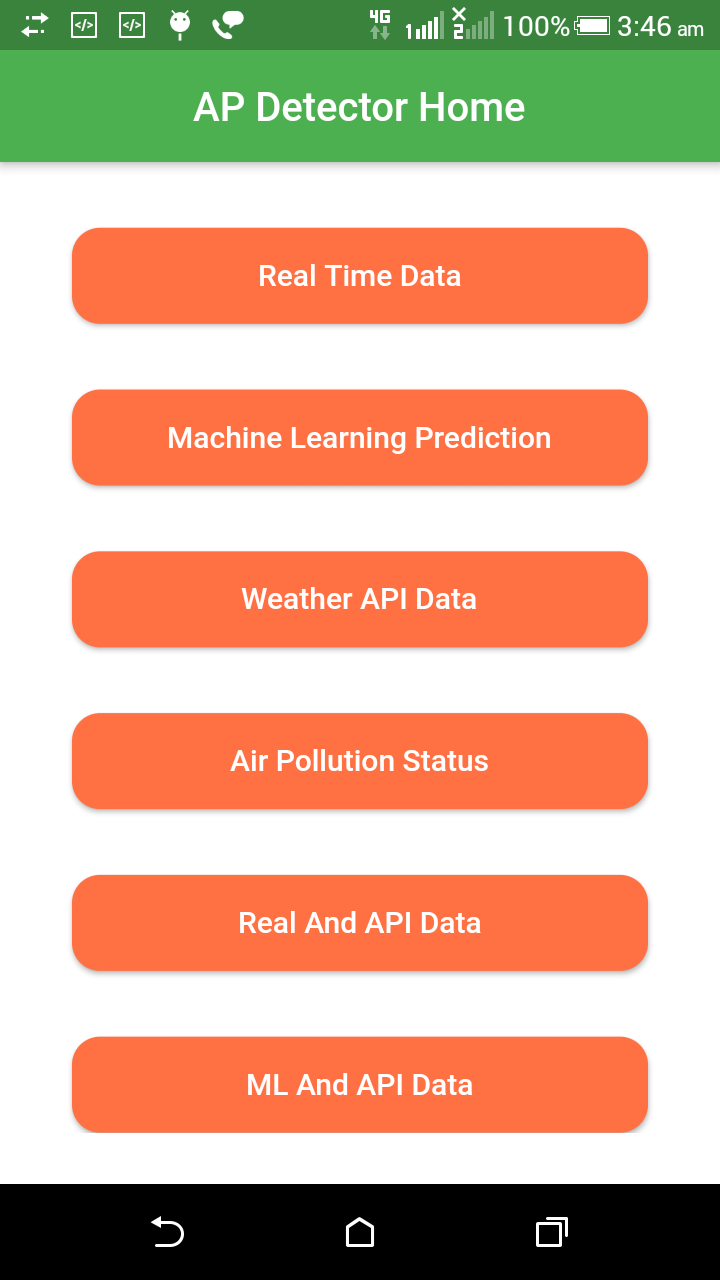
\includegraphics[height=10cm]{figures/home-screen.png}
\caption{\label{img414} Application home screen}
\end{figure}

\subsection{Real Time Data}
When will be pressing on first RadioButton then will go to figure~\ref{img415} screenshot page basically this page is showing real time data that are coming from all gas sensors and temperature sensor.

\begin{figure}[!ht]
\centering
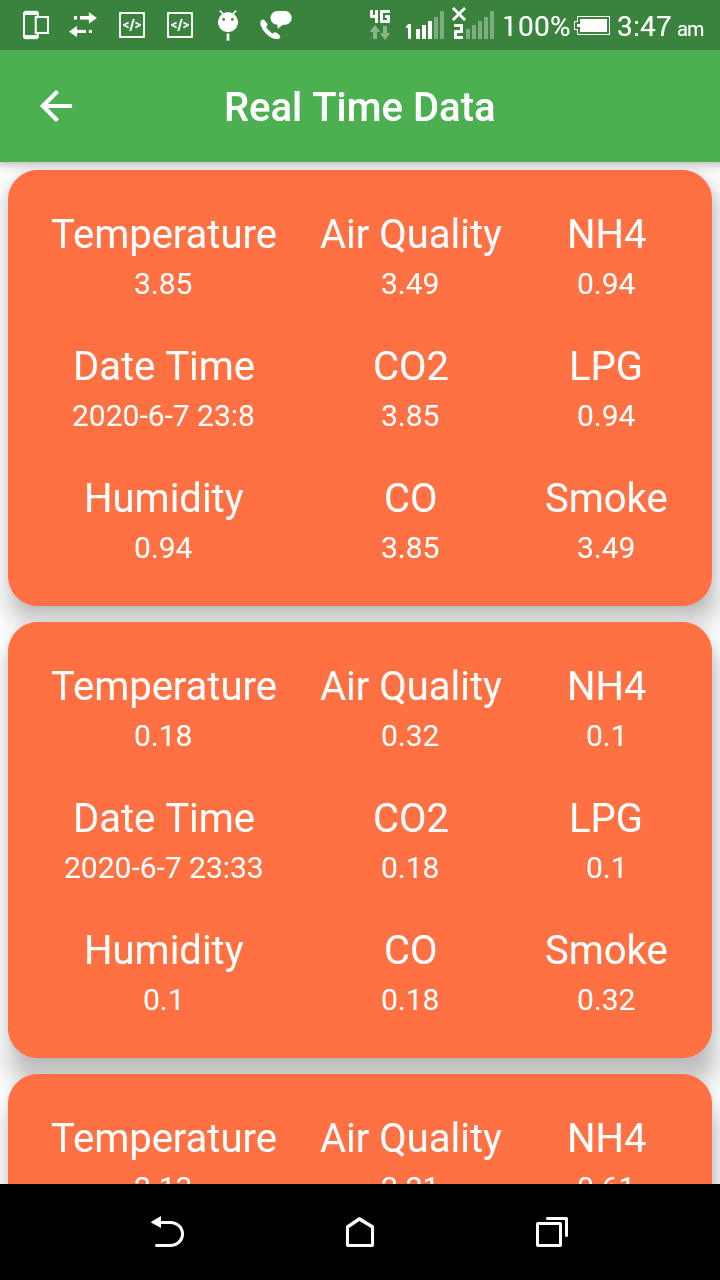
\includegraphics[height=10cm]{figures/real-data.png}
\caption{\label{img415} Real time data page}
\end{figure}

\subsection{ML Prediction Data}
When will be pressing on second RadioButton then will go to figure~\ref{img416} screenshot page basically this page is showing machine learning model prediction data that are coming from server. This page has next five day's weather forecast record which is after every 3 hours interval from current time. 

\begin{figure}[!ht]
\centering
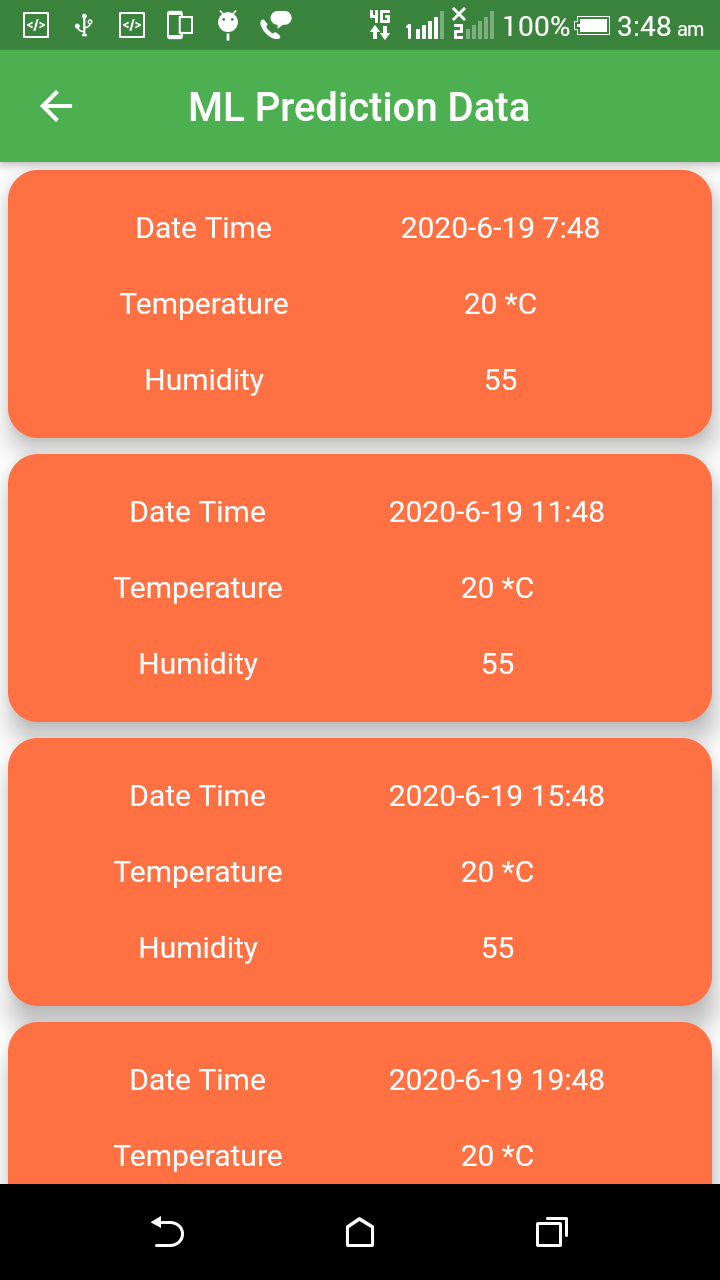
\includegraphics[height=10cm]{figures/ml-data.png}
\caption{\label{img416} ML prediction data page}
\end{figure}

\subsection{Weather API Data}
When will be pressing on third RadioButton then will go to figure~\ref{img417} screenshot page basically this page has two input field which are for latitude and longitude of current location, two RadioButtons first for current weather details and second for next five day's weather forecast and last one output field for showing details after pressing above two buttons.

\begin{figure}[!ht]
\centering
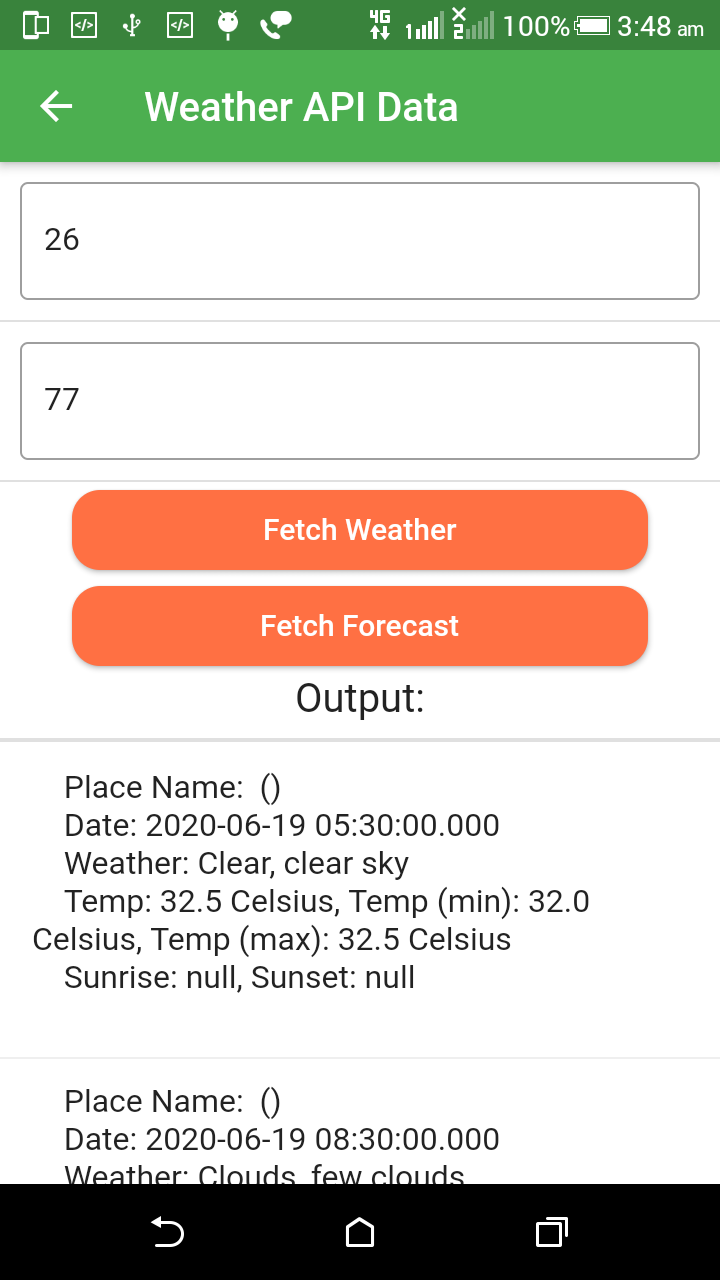
\includegraphics[height=10cm]{figures/weather-data.png}
\caption{\label{img417} Weather API data page}
\end{figure}

\subsection{Air Pollution Status}
When will be pressing on fourth RadioButton then will go to figure~\ref{img418} screenshot page basically this page is showing eight graphs that are temperature, humidity, air quality, carbon monoxide(CO), carbon dioxide($CO_{2}$),ammonium($NH_{4}$), smoke and LGP gas with respect to time.

\begin{figure}[!ht]
\centering
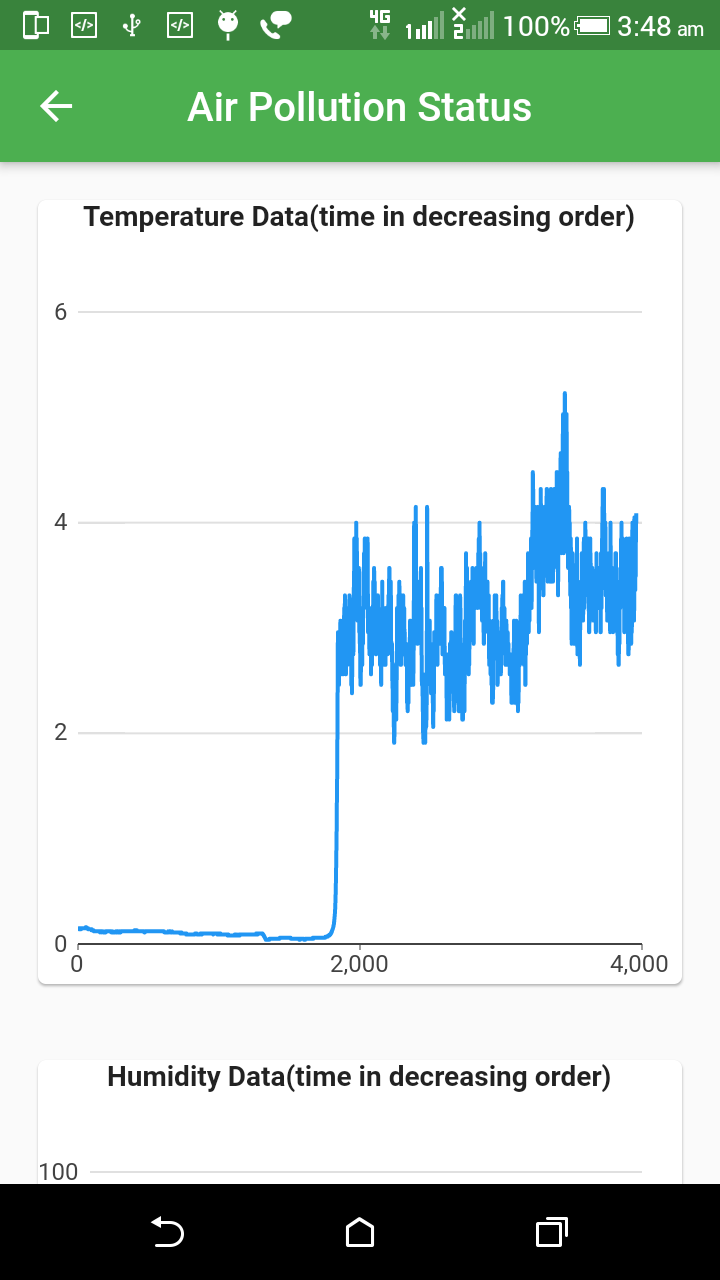
\includegraphics[height=10cm]{figures/pollution-status.png}
\caption{\label{img418} Weather API data page}
\end{figure}









% \label{chap4:intro}
% Research~\cite{wells+92} in science and technology has played a vital role in improvising human life at great extent. With the development of instrumentation and computation facilities, research on frontier areas has gone manifold. The discussion on the frontier areas of research in inter- disciplinary subject has always yielded novel ideas and collaborative research.


% \begin{figure}[!ht]
% \centering
% \includegraphics[scale=0.9]{car1.png}
% \caption{\label{img3} Image caption}
% \end{figure}

% Research in science and technology has played a vital role in improvising human life at great extent. With the development of instrumentation and computation facilities, research on frontier areas has gone manifold. The discussion on the frontier areas of research in inter- disciplinary subject has always yielded novel ideas and collaborative research. 

% \subsection{Test cases}
% Research in science and technology has played a vital role in improvising human life at great extent. With the development of instrumentation and computation facilities, research on frontier areas has gone manifold. The discussion on the frontier areas of research in inter- disciplinary subject has always yielded novel ideas and collaborative research.  








% %+++++++++++++++++++++++++++++++++++++++++++++++++++++++++++++++++++++++++++++++++
% \section{Summary}
% \label{chap4:sum}
% Research in science and technology has played a vital role in improvising human life at great extent. With the development of instrumentation and computation facilities, research on frontier areas has gone manifold. The discussion on the frontier areas of research in inter- disciplinary subject has always yielded novel ideas and collaborative research. In view of this, the First International Conference on Smart Technologies in Computer and Communication (SmartTech-2017) is meticulously planned to muster innovative ideas from researchers, scientists, academicians, Industry professionals and students. The aim of the conference is to provide a common platform to share and discuss the novel ideas, technologies and research findings to promote interdisciplinary research and to ignite young brains.


 %Implementation
\chapter{Conclusion} \label{chap5}
\thispagestyle{empty}


\vspace*{40 ex}
%============================================================


This research proposed a smart air pollution monitoring system that constantly keeps track of air quality in an area and sends data into cloud storage and also displays the air quality measured on Flutter Application in real time. The environment data which this monitoring system is sensing, contains the label of various gases such as carbon monoxide(CO), carbon dioxide($CO_{2}$), ammonium($NH_{4}$), Liquefied petroleum gas(LPG), air quality index(AQI) and smoke and other parameters like temperature, humidity and many more. The beauty of this proposed system is that we can see real time data of the location where this system is setup through all around world.

The second important feature of this monitoring system, it shows weather forecast of next 5 days from current time. The forecasting contains temperature, humidity and pressure and it does six predictions in a day(i.e after every 3 hours).

The third important feature of this monitoring system, it alarms to the people for the weather condition both depend on current real time data and also feature prediction if the label goes up to decided threshold then it alarms to it's user.

The four important feature of this monitoring system, it shows a detail analysis of data by plotting graph to each and every part of data with respect to time.

The fifth and last important feature of this monitoring system, it shows current data of weather API and next 5 days weather forecast depend on Geolocation(i.e latitude and longitude).

The system helps to create awareness of the quality of air that one breathes daily. This monitoring device can be delivered real-time measurements of air quality in national level. If air quality is less than 500 ppm then it is fresh air and if it is between 1000 ppm to 2000 ppm then it is poor air quality we should open the windows of the room and at last if it is greater than 2000 ppm then it is danger the area is very much polluted. When we start sensing air and noise pollution the area where we placed our air and sound come under the range where air quality is in between 200ppm to 750 ppm it comes under fresh air quality region.



\section{Future direction}
The project is intended victimization structured modeling and is ready to supply the
required results. It is with success enforced as a true Time system with bound
modifications. Science is discovering or making major breakthrough in varied fields, and thus technology keeps dynamic from time to time. Going more, most of the units is fictional on one in conjunction with microcontroller so creating the system compact thereby creating the present system simpler.

To make the system applicable for real time functions parts with larger vary must be
enforced. This system is any enlarged to observe the developing cities and industrial zones for pollution monitoring. To safeguard the general public health from pollution, this system provides associate economical and low price resolution for continuous observance of atmosphere.

In future we may be extended to this system include features such as:
\begin{itemize}
\item Shifting from Raspberry PI to some low cost microcontroller
\item Adding more sensors to get more detailed air quality
\item Adding new model so that it can predict more features such as windspeed, airdirection, etc.
\item Adding more features in flutter applications such as bar charts, histogram analyzes data in more detail
\end{itemize}


 %Conclusion
\end{onehalfspace}

\begin{singlespace}
\begin{appendices}
\chapter{Screenshots}\label{appendix1}

%##########################################

\begin{figure}[!ht]
\centering
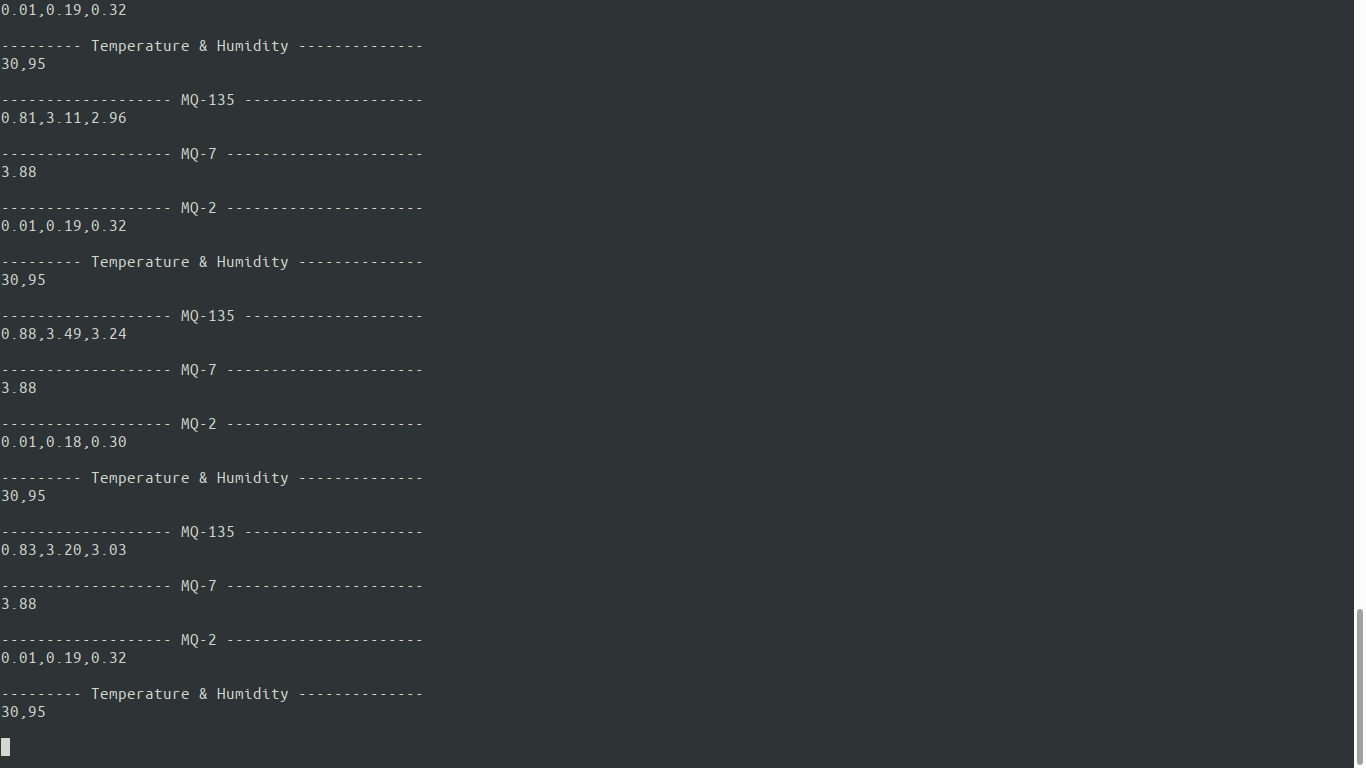
\includegraphics[width=\linewidth]{figures/clt-data.png}
\caption{\label{imgA2} CLI data that's coming from Arduino UNO}
\end{figure}

\begin{figure}[!ht]
\centering
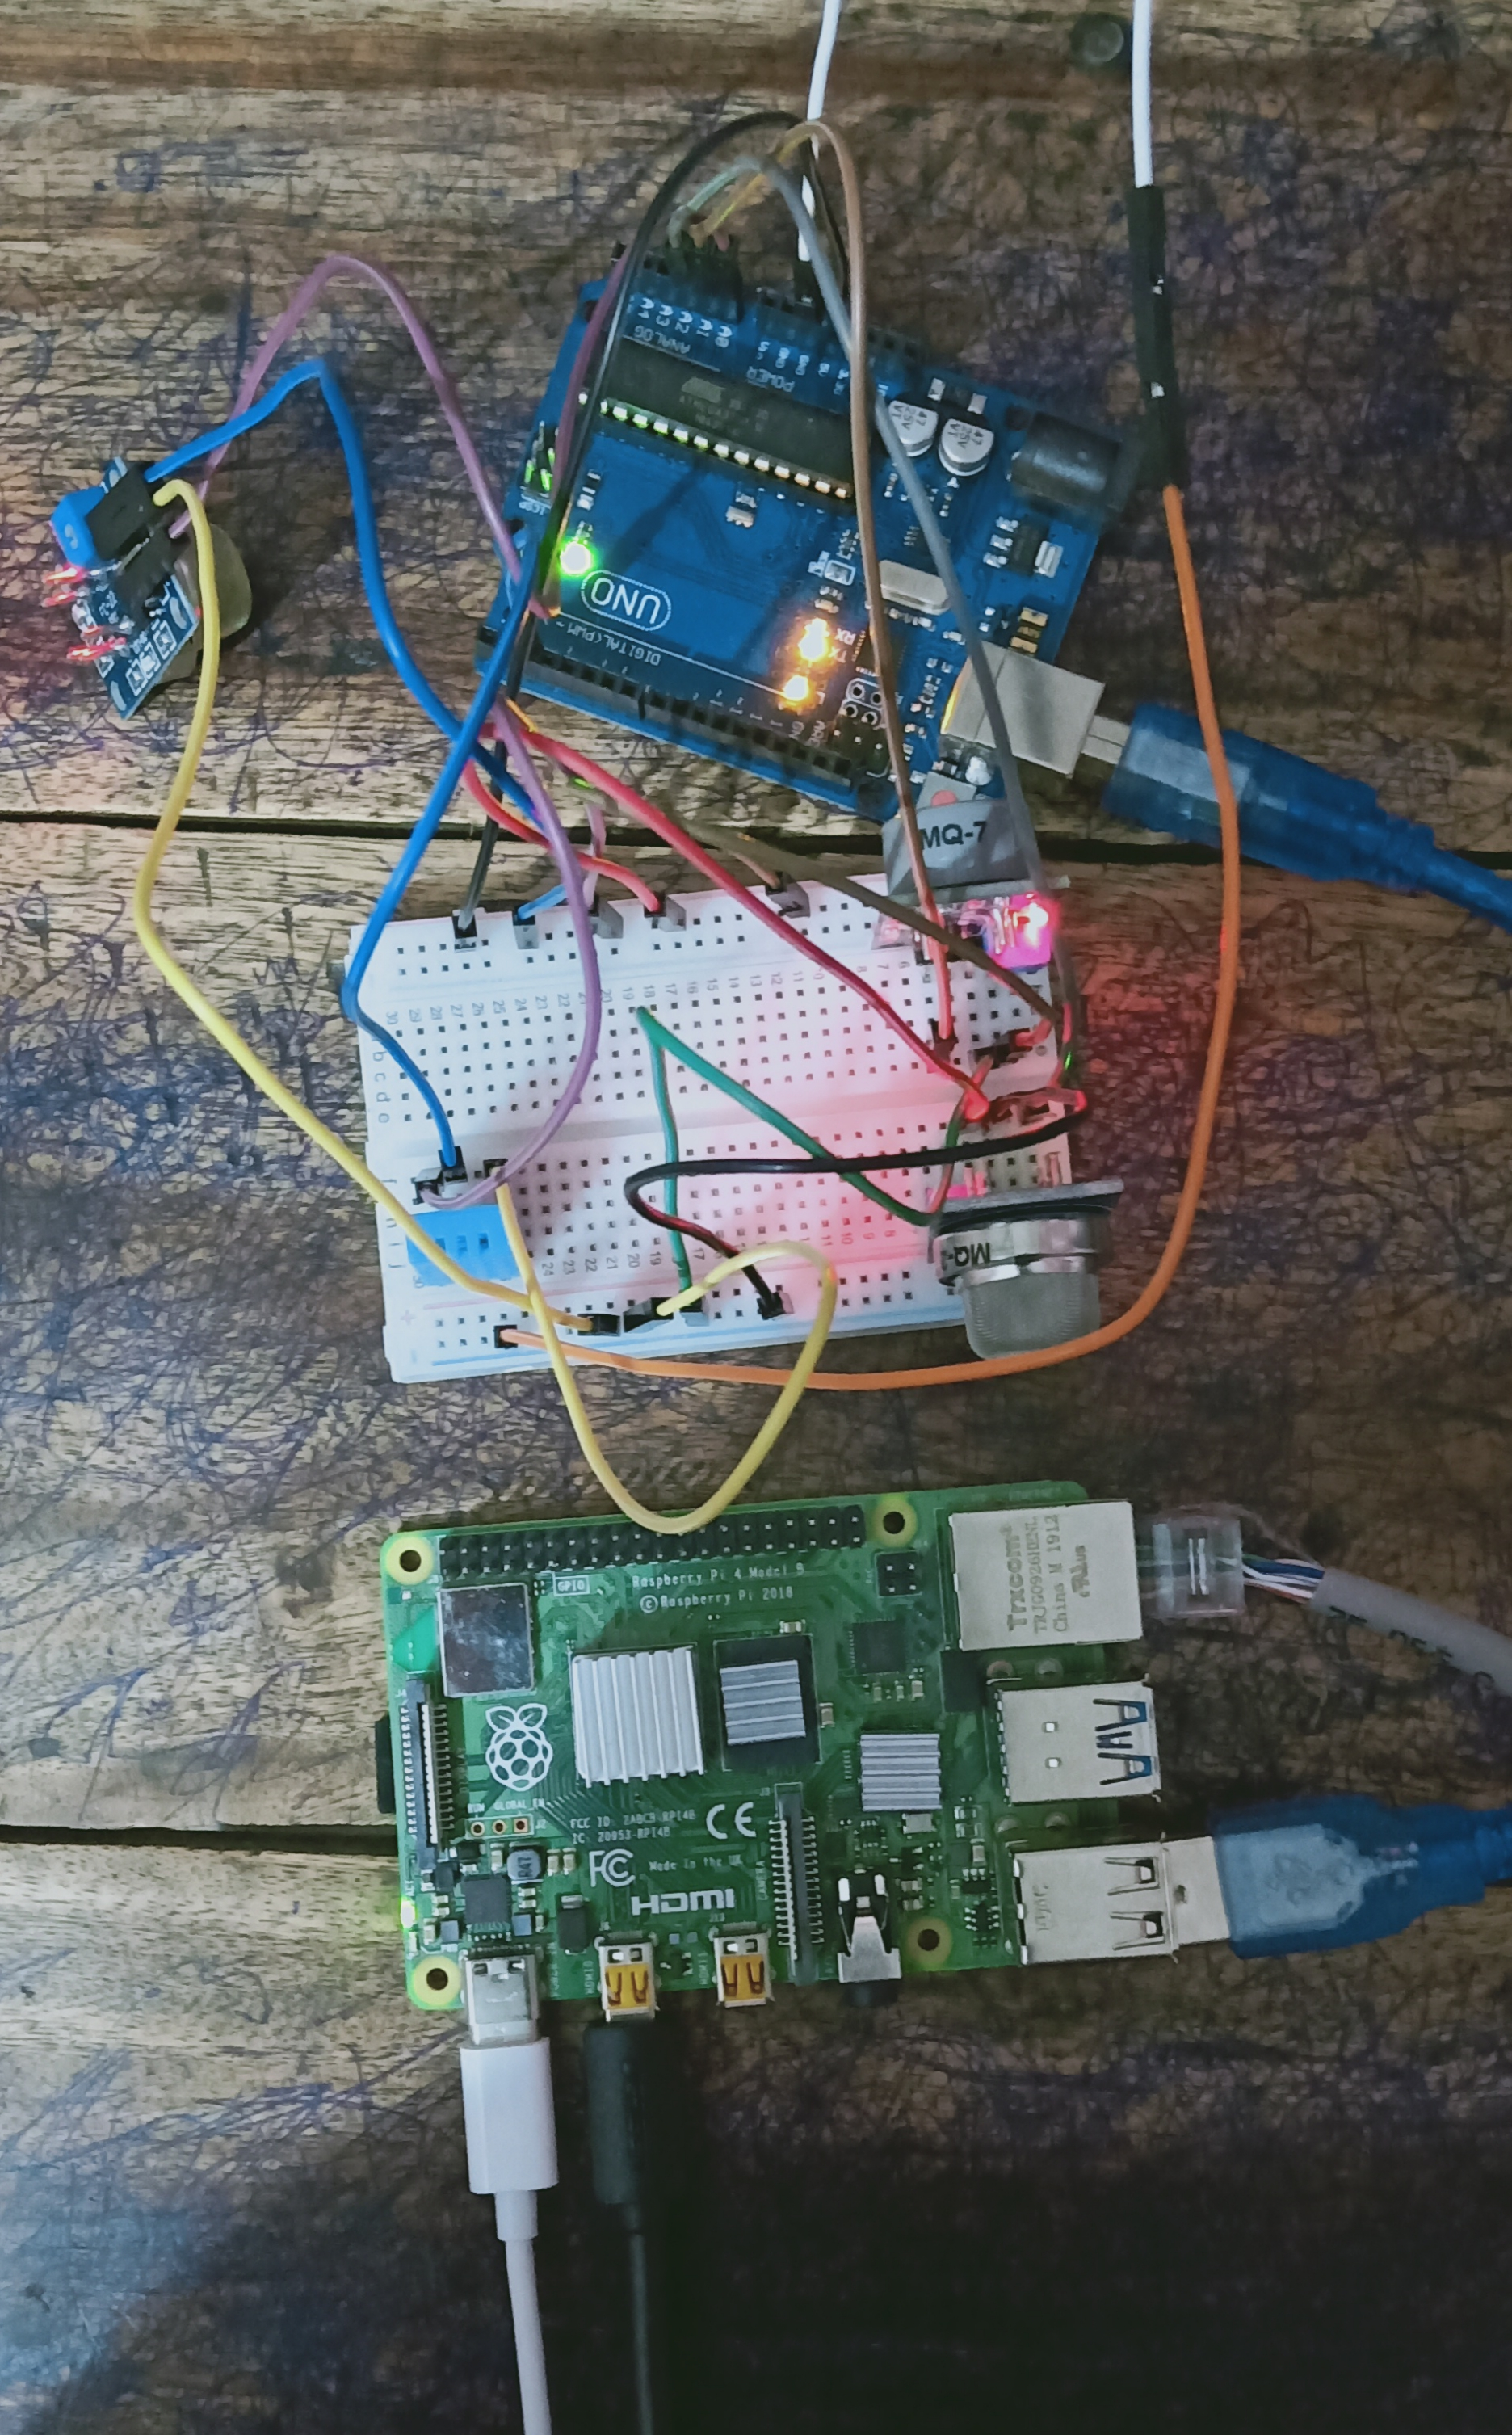
\includegraphics[width=\linewidth,height = 20cm]{figures/hardware.jpg}
\caption{\label{imgA1} Complete hardware setup}
\end{figure}


\chapter{User manual}\label{appendix2}

%##########################################


\section{System Specification}

\subsection{Hardware Requirement}

\subsubsection{Android}
\begin{itemize}
\item Android Version should be greater than 5.1(i.e API 22)
\item Ram- minimum :- 512 MB
\item Hard disk—minimum :- 5 GB
\item Processor :- Qualcomm’s Snapdragon 545 or other processor with relative power
\end{itemize}

\subsubsection{iOS}
\begin{itemize}
\item iOS Version should be greater than 8
\item Ram- minimum :- 512 MB
\item Hard disk—minimum :- 5 GB
\item Processor :- Qualcomm’s Snapdragon 545 or other processor with relative power
\end{itemize}


\subsection{Software Requirement}

There is no software requirement for this application because Android and iOS have in-build all Software requirement. There is nothing to do with this application just take APK file to your Android device or IPA file for your iOS device and install it.


\section{Step to install this application}
All the part of data calibration, data storage, model creation, model deployment, weather forecast prediction, flutter application is done by developer side user don't have to worry about any dependency and other installation, all user needs to do, just take given file for Android or iOS and install it into their device.

\subsection{Android}
Installation process is very easy, there is nothing to do with this just get APK file(i.e app-release.apk) and install to your Android device, installation will be taking hardly 1-2 minutes and installation user will be able to use this application.

\subsection{iOS}
Installation process is very easy, there is nothing to do with this just get IPA file(i.e app-release.ipa) and install to your iOS device, installation will be taking hardly 1-2 minutes and installation user will be able to use this application.
\end{appendices}
\end{singlespace}
\thispagestyle{empty}




\begin{onehalfspace}
\cleardoublepage\phantomsection\addcontentsline{toc}{chapter}{Bibliography}
\nocite{*}
\bibliographystyle{IEEEtran}
\bibliography{project}
\end{onehalfspace}



\newpage
\addcontentsline{toc}{chapter}{\numberline{}Index}
\singlespacing{\printindex}

\end{document}





